\documentclass[nostrict]{szablonPG}

\usepackage{listing_schemat}
\usepackage{tikz}
\usetikzlibrary{matrix,chains,positioning,decorations.pathreplacing,arrows}

\begin{document}

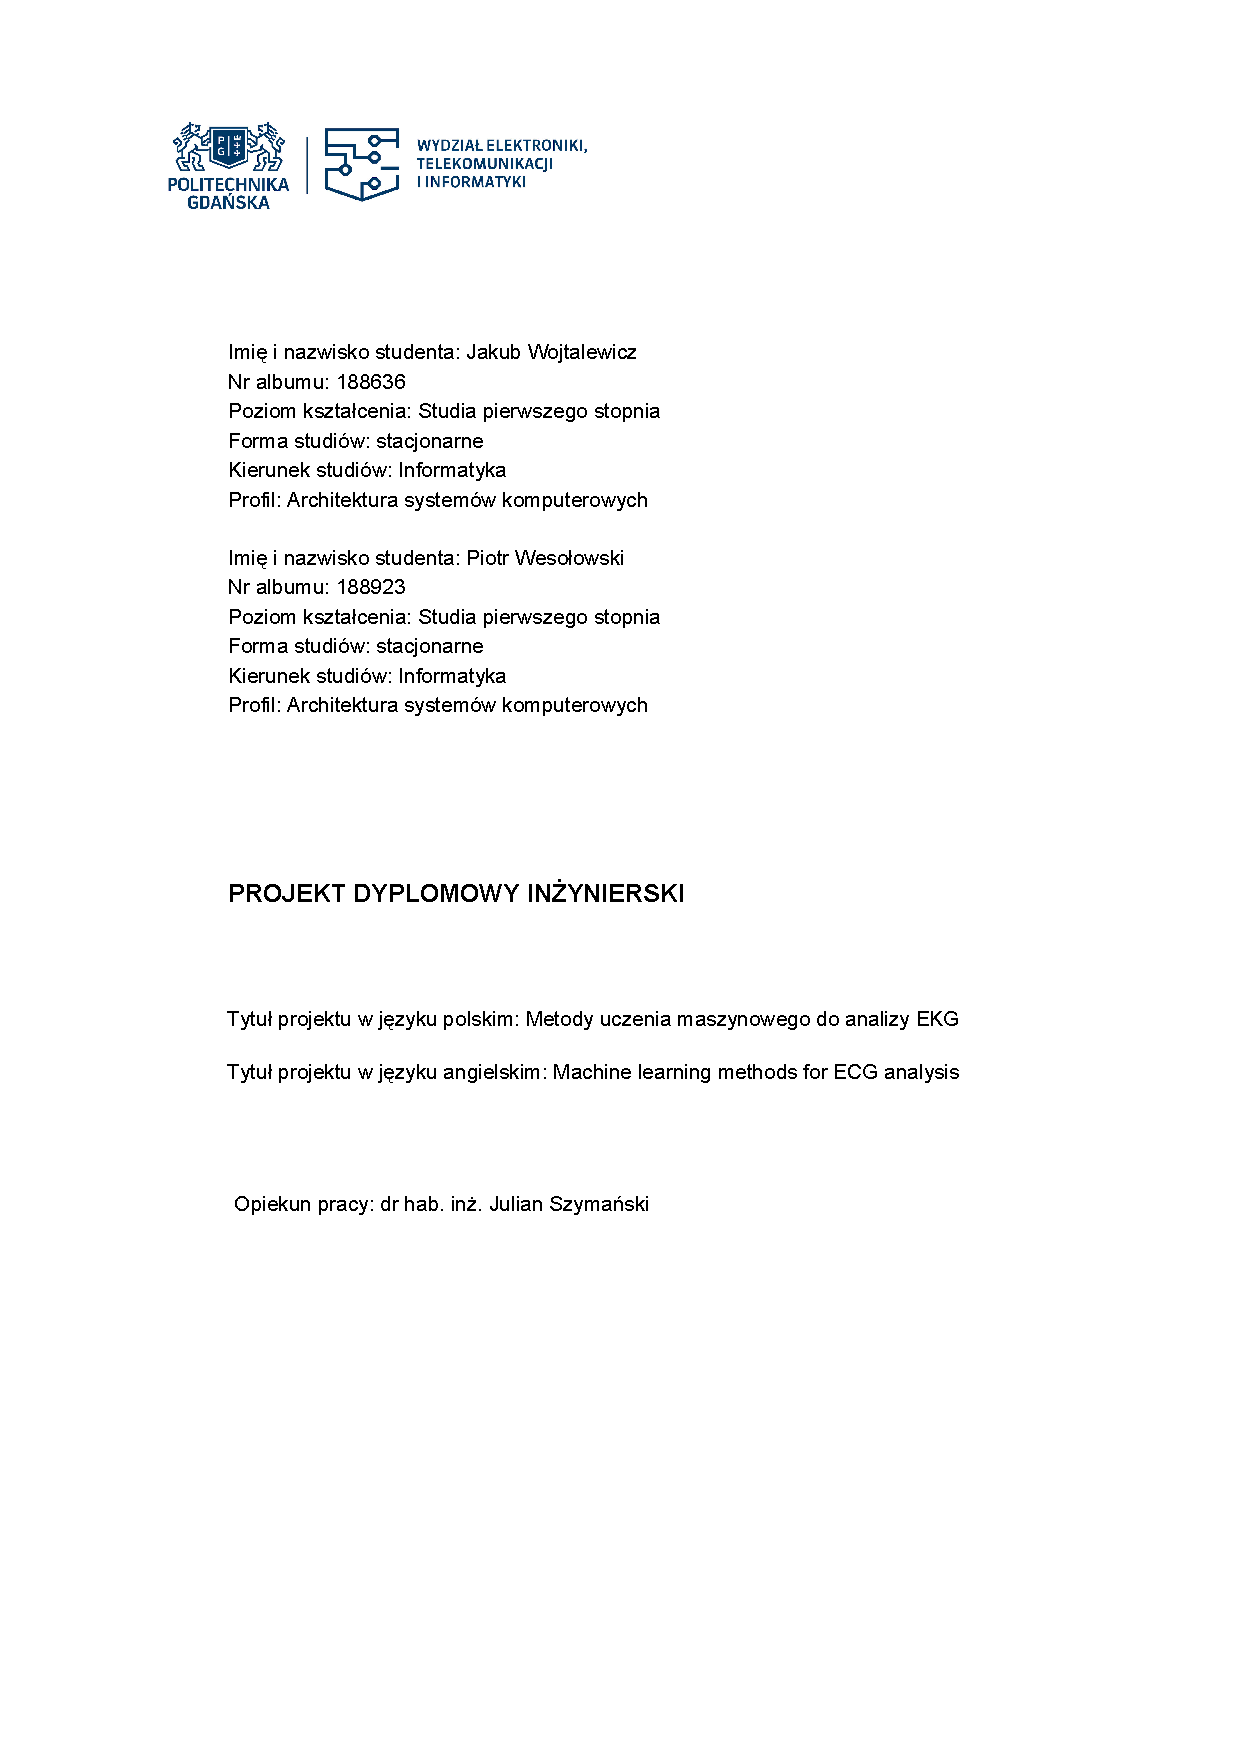
\includepdf{meta/StronaTytulowa.pdf}
\chapter*{Streszczenie}
\indent Lorem Lorem ipsum dolor sit amet, consectetur adipiscing elit. Vivamus elementum arcu nec blandit aliquam. Integer eros dolor, molestie eget dictum quis, luctus sit amet sapien. Proin dignissim felis in ornare volutpat. Morbi vulputate rutrum efficitur. Ut vehicula vehicula metus, et iaculis tortor mattis vel. Nam blandit, arcu quis ultricies blandit, libero ante commodo augue, in accumsan dui leo at orci. Phasellus in augue et velit pulvinar malesuada ut et sem. Nulla vehicula nibh eu odio sollicitudin sagittis. Praesent condimentum semper neque, tincidunt luctus nisl scelerisque sed. Orci varius natoque penatibus et magnis dis parturient montes, nascetur ridiculus mus. 
\vspace{0.5cm}\newline
\textbf{S�owa kluczowe:} lorem ipsum, dolor sit amet, consectetur adipiscing\vspace{0.5cm}

\noindent \textbf{Dziedzina nauki i techniki, zgodnie z wymogami OECD:} nauki in�ynieryjne i techniczne, robotyka i automatyka

\chapter*{Abstract \small{(author: Piotr Wesołowski)}}
\indent The engineering thesis presents a system for analyzing ECG signals using machine learning methods, focusing on heart rate variability (HRV) and the respiratory sinus arrhythmia (RSA) effect. The project is based on real-time data processing using the Polar H10 sensor and a dedicated application that enables the acquisition of ECG signals transmitted via Bluetooth. The system also supports the analysis of complete signal datasets loaded from files, allowing for comprehensive investigation of data dependencies.

The system implements various data analysis techniques, each requiring the prior identification of characteristic peaks in the ECG signal using a custom-developed algorithm. Based on the detected peaks, intervals between them were calculated, forming the foundation for further analysis. The primary analysis, performed in the time domain, allowed for the calculation of several key metrics based on these intervals. These intervals were also utilized in frequency and time-frequency analyses. Advanced mathematical transformations, such as the Fast Fourier Transform and wavelet analysis, were applied in these methods. The results of the analyses related to heart rate variability are presented as numerical values of key metrics and their time-varying characteristics on clear visual graphs.

The thesis compares the effectiveness of a traditional algorithm for R-peak detection with a machine learning-based algorithm. The applied neural networks achieved high accuracy in detecting characteristic peaks in the ECG signal and predicting various heart rate variability metrics based on them. An innovative approach was developed, enabling the prediction of HRV and RSA parameters directly from the entire ECG signal, representing a significant extension of the traditional RR-interval-based approach.

The thesis experimentally examined the impact of breathing patterns on RSA and analyzed the diurnal variability of heart activity by comparing differences between daytime and nighttime. A qualitative analysis of the developed neural network models was also conducted, highlighting their strengths, potential development directions, and possible applications in biomedical data analysis.

The system and methods presented in this thesis constitute a comprehensive platform for ECG analysis, with potential applications in scientific research and medical diagnostics.
\vspace{0.5cm}\newline
\textbf{Keywords:} Machine learning, EKG, HRV, RSA, Polar H10, end-to-end analysis \vspace{0.5cm}

\tableofcontents

\chapter{Wprowadzenie i cel pracy \small(autor: Piotr Weso�owski)}
Elektrokardiografia (EKG) to kluczowe narz�dzie diagnostyczne w analizie pracy serca, pozwalaj�ce na wykrywanie wielu nieprawid�owo�ci, b�d�cych jedn� z g��wnych przyczyn zgon�w na �wiecie \cite{Coronado-CVD-Global}. Poprawna analiza sygna�u EKG jest zadaniem niezwykle skomplikowanym i mimo licznych bada� w tym zakresie wci�� rozwijane s� nowe metody i podej�cia. Dzi�ki cyfrowemu zapisowi sygna�u serca mo�na stosowa� zaawansowane metody przetwarzania danych w analizie czasowej, cz�stotliwo�ciowej i nieliniowej. Rozwi�zanie to pozwala dostrzec r�nice, kt�re mog� pozosta� niewykryte podczas wizualnej analizy sygna�u przedstawionego na tradycyjnym wykresie na papierze milimetrowym.

Nowoczesne techniki analizy, takie jak eksploracja danych (data mining), pozwalaj� na uproszczenie monitorowania pracy serca w por�wnaniu z tradycyjnymi metodami. Z kolei metody uczenia maszynowego umo�liwiaj� wzrost efektywno�ci analizy sygna��w zaszumionych, kt�re stanowi� nieod��czny element d�u�szych rejestracji sygna�u. Podej�cie to eliminuje konieczno�� r�cznej korekcji, co jest czasoch�onne w klasycznych podej�ciach. Szczeg�lnym ich przyk�adem s� rozwi�zania end-to-end, oparte na analizie ca�ego sygna�u, kt�re pozwalaj� na tworzenie uniwersalnych modeli niezale�nie od aktualnie rozpatrywanego problemu. Tego rodzaju podej�cie wci�� nie jest zbyt szeroko opisane w literaturze naukowej, co stwarza przestrze� dla nowych bada� w tym zakresie.

W niniejszej pracy skupiono si� na wykorzystaniu zaawansowanych metod analitycznych, w tym sieci neuronowych, do analizy sygna�u EKG. G��wnym celem by�o opracowanie algorytmu umo�liwiaj�cego w czasie rzeczywistym wykrywanie kluczowych wzorc�w (np. za�amk�w R) oraz obliczanie wska�nik�w zmienno�ci rytmu serca (HRV) i analizy arytmii oddechowej (RSA). Opracowanie takiego rozwi�zania pozwala na kompleksow� i precyzyjn� analiz� sygna�u EKG zar�wno w badaniach naukowych, jak i w codziennej praktyce klinicznej.

\chapter{Podstawy teoretyczne}
Rozdzia� ten stanowi wprowadzenie teoretyczne do tematyki pracy, omawiaj�c
podstawowe poj�cia i kluczowe aspekty zwi�zane z analiz� sygna��w EKG, kt�re s�
istotne dla zrozumienia dalszych cz�ci opracowania. Przedstawiono tutaj og�lne za�o�enia dzia�ania elektrokardiografii, opis kluczowych sk�adowych sygna�u EKG oraz podstawowe parametry wykorzystywane w analizie zmienno�ci rytmu serca. Dokonano r�wnie� przegl�du metod uczenia maszynowego wykorzystywych w literaturze
naukowej do analizy sygna��w EKG.

\section{Elektrokardiografia \small{(autor: Jakub Wojtalewicz)}}

Elektrokardiografia, w skr�cie EKG, to badanie polegaj�ce na rejestracji
aktywno�ci elektrycznej serca. Zazwyczaj przyjmuje form� graficznego wykresu,
przedstawiaj�cego zmiany potencja��w elektrycznych serca w czasie
\cite{Lilly-Pathophysiology}. Rejestracja odbywa sie za pomoc� elektrod 
umieszczonych na ciele pacjenta w okre�lonych miejscach, takich jak klatka
piersiowa oraz ko�czyny, co pozwala na wychwycenie sygna��w bioelektrycznych
generowanych przez mi�sie� sercowy podczas jego pracy \cite{Romano-ECG}.

Badanie EKG jest istotnym narz�dziem diagnostycznym w medycynie przez swoj�
nieinwazyjno�� oraz pr�dko�� wykonania. Umo�liwia wykwalifikowanym lekarzom
ocen� stanu uk�adu sercowo-naczyniowego pacjenta oraz rozpoznanie wyst�puj�cych
nieprawid�owo�ci, kt�re mog� by� spowodowane wszelakimi schorzeniami
\cite{Malik-HRV}.

\section{Sk�adowe sygna�u EKG \small{(autor: Jakub Wojtalewicz)}}

% Sygna� EKG sk�ada si� z cyklicznie powtarzaj�cych si� fal i segment�w, kt�re odzwierciedlaj� r�ne fazy pracy serca. Cykl serca zaczyna sie za�amkiem P, odpowiadaj�cym za depolaryzacj� przedsionk�w serca, prowadz�cej do ich skurczu. Po nim nast�puje kompleks QRS, kt�ry jest odpowiedzialny za depolaryzacj� kom�r serca - kluczowego momentu skurczu mi�nia. Kompleks sk�ada sie z trzech fal: za�amka Q - pierwszego negatywnego w kompleksie - przedstawiaj�cego rozchodzenie si� impulsu elektrycznego w przegrodzie mi�dzykomorowej. Po nim nast�puje za�amek R - dodatni, zazwyczaj najbadziej widoczny komponent kompleksu - odzwierciedlaj�cy g�own� faz� depolaryzacji, kiedy wi�kszo�c masy mi�sniowej kom�r jest pobudzana do skurczu. Kompleks ko�czy kolejny za�amek negatywny S, reprezentuj�cy ko�cow� faz� depolaryzacji - na wykresie charakteryzuje go spadek poni�ej linii izoelektrycznej, bazowej wykresu. 

Sygna� EKG sk�ada si� z cyklicznie powtarzaj�cych si� fal i segment�w, kt�re
odzwierciedlaj� r�ne fazy pracy serca. Typowo segmenty te s� oznaczane kolejno
jako \textbf{P-QRS-T} Rys. \ref{fig/ekgGraph}. Cykl serca rozpoczyna si�
za�amkiem P, kt�ry odpowiada za depolaryzacj� przedsionk�w, prowadz�c� do ich
skurczu. Nast�pnie wyst�puje kompleks QRS, odpowiedzialny za depolaryzacj�
kom�r serca � kluczowy moment skurczu mi�nia sercowego. Kompleks ten sk�ada
si� z trzech fal:

\begin{itemize}
    \item \textbf{Za�amek Q} to pierwszy negatywny za�amek w kompleksie, kt�ry odzwierciedla pocz�tkow� faz� rozchodzenia si� impulsu elektrycznego przez przegrod� mi�dzykomorow�.
    \item \textbf{Za�amek R} jest dodatni i najcz�ciej najwi�kszy w ca�ym kompleksie. Reprezentuje g��wn� faz� depolaryzacji kom�r, kiedy wi�kszo�� masy mi�niowej zostaje pobudzona do skurczu.
    \item \textbf{Za�amek S} to kolejny negatywny za�amek, kt�ry zamyka kompleks QRS i reprezentuje ko�cow� faz� depolaryzacji kom�r, widoczn� jako spadek wykresu poni�ej linii izoelektrycznej.
\end{itemize}

Po kompleksie QRS pojawia si� za�amek T, kt�ry obrazuje repolaryzacj� kom�r,
czyli powr�t mi�nia sercowego do stanu spoczynkowego po skurczu. Za�amek T
jest zwykle dodatni i mniej wyra�ny ni� za�amek R, lecz jego kszta�t, czas
trwania oraz amplituda maj� istotne znaczenie diagnostyczne. Nieprawid�owo�ci w
za�amku T mog� wskazywa� na problemy takie jak niedokrwienie mi�nia sercowego,
zaburzenia elektrolitowe lub inne patologie repolaryzacyjne.

Ca�y cykl serca przedstawiony w sygnale EKG odzwierciedla skoordynowane zmiany
elektryczne zachodz�ce w sercu, dostarczaj�c szczeg�owych informacji o jego
funkcjonowaniu. Ka�dy komponent ma kluczowe znaczenie diagnostyczne,
umo�liwiaj�c ocen� stanu uk�adu sercowo-naczyniowego oraz identyfikacj�
r�norodnych zaburze� i patologii sercowych \cite{Romano-ECG}.

\begin{figure}[ht]
    \centering
    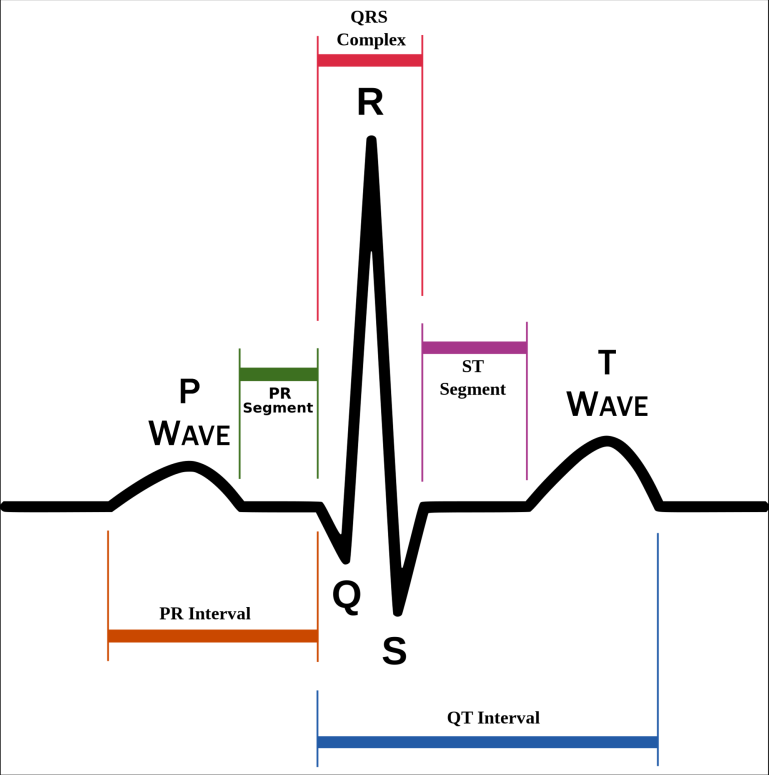
\includegraphics[scale=0.25]{Rysunki/Normal-ECG-signal-with-his-different-features.png}
    \caption{Normalny sygna� EKG z jego cechami.}
    \caption*{�r�d�o:  \url{https://www.researchgate.net/figure/Normal-ECG-signal-with-his-different-features_fig1_299575422} [Data uzyskania dost�pu 02.11.2024]}
    \label{fig/ekgGraph}
\end{figure}

\section{Charakterystyki sygna�u EKG \small{(autor: Piotr Weso�owski)}}\label{MiaryHRV}

Podczas analizy sygna�u EKG wyr�ni� mo�na wiele charakterystyk, kt�re
dostarczaj� szczeg�owych informacji o pracy serca i kondycji uk�adu
sercowo-naczyniowego badanej osoby.

\subsection{Odst�py RR i puls}

Jednym z kluczowych parametr�w opisuj�cych sygna� EKG jest czas pomi�dzy kolejnymi szczytami za�amk�w R, wyra�any w milisekundach (ms). Parametr ten nazywany jest \textit{odst�pem RR} (ang. \textit{RR interval}). W literaturze wyst�puje r�wnie� okre�lenie \textit{odst�p NN} (ang. \textit{NN interval}), kt�re odnosi si� do odst�p�w pomi�dzy kolejnymi za�amkami R, ale z uwzgl�dnieniem wy��cznie rytmu prawid�owego, pozbawionego artefakt�w i zak��ce� (ang. \textit{normal-to-normal}). Chocia� w praktyce oba terminy bywaj� u�ywane zamiennie, w analizach dotycz�cych pracy serca kluczowe jest, aby uwzgl�dnia� jedynie prawid�owy rytm, wolny od znacz�cych zak��ce� i artefakt�w. Jego analiza pozwala bezpo�rednio okre�li� inn� istotn� metryk�, jak� jest puls, czyli \textit{HR} (ang. \textit{heart rate}), kt�ry oznacza liczb� uderze� serca na minut�. Ka�demu skurczowi serca towarzyszy charakterystyczny wzrost potencja�u elektrycznego, rejestrowany jako szczyt $R$ na wykresie EKG \cite{Zhan-RWave}.

Chwilowe t�tno w chwili \( t_{R_n} \), czyli w momencie wyst�pienia \( n \)-tego szczytu \( R \), mo�na wyrazi� za pomoc� wzoru:

\begin{equation}  
    HR_n = \frac{60}{t_{R_n} - t_{R_{n-1}}}
\end{equation}

gdzie:

\begin{itemize}
    \item \( t_{R_n} \) to czas wyst�pienia \( n \)-tego szczytu \( R \),
    \item \( t_{R_{n-1}} \) to czas wyst�pienia poprzedniego szczytu \( R \),
    \item wynik \( HR_n \) wyra�ony jest w uderzeniach na minut� (bpm, \textit{beats per minute}).\\
\end{itemize}



Je�li jednak chcieliby�my przybli�y� warto�� t�tna w dowolnym punkcie pomi�dzy szczytami, nale�a�oby t� warto�� odpowiednio ekstrapolowa�.

Wielko�� r�nic pomi�dzy kolejnymi odst�pami RR (tzw. \textit{RR variability}) jest kolejnym kluczowym wska�nikiem pracy serca. Analiza tych r�nic, wykorzystuj�c miary czasowe i cz�stotliwo�ciowe, jest podstaw� do okre�lenia zmienno�ci rytmu serca, szeroko opisywanej w dalszej cz�ci tej pracy.


\subsection{Analiza w domenie czasowej}

Metody analizy czasowej opieraj� si� na bezpo�rednim pomiarze odst�p�w RR w sygnale EKG, kt�re reprezentuj� czas mi�dzy kolejnymi skurczami serca. Poni�ej przedstawiono podstawowe miary analizy czasowej:

\subsubsection{SDNN} \label{SDNN}
{SDNN} (ang. \textit{Standard Deviation of NN intervals}), czyli odchylenie standardowe wszystkich odst�p�w RR w badanym okresie, jest jedn� z podstawowych miar zmienno�ci rytmu serca. Warto�� SDNN odzwierciedla ca�kowit� zmienno�� sygna�u rytmu serca, poniewa� wariancja sygna�u, b�d�ca kwadratem odchylenia standardowego, jest r�wna sumie mocy w ca�ym zakresie cz�stotliwo�ci \cite{Saul1988}. SDNN jest prost� miar� do obliczenia, jednak nie jest dobrze zdefiniowan� zmienn� statystyczn�, poniewa� jej warto�� zale�y od d�ugo�ci badania. Wielko�� SDNN wzrasta wraz z czasem trwania rejestracji, dlatego por�wnywanie wynik�w mi�dzy badaniami o r�nej d�ugo�ci wymaga wcze�niejszej normalizacji do okre�lonych okres�w, np. do nominalnych zapis�w 24-godzinnych lub kr�tkoterminowych trwaj�cych 5 minut.

\begin{equation}
  \text{SDNN} = \sqrt{\frac{1}{N-1} \sum_{i=1}^{N} \left( RR_i - \overline{RR} \right)^2}
\end{equation}

gdzie:

\begin{itemize}
  \item \(RR_i\) to kolejne odst�py RR (czas mi�dzy kolejnymi uderzeniami serca),
  \item \(\overline{RR}\) to �rednia warto�� odst�p�w RR,
  \item \(N\) to liczba wszystkich pomiar�w odst�p�w RR, czyli liczba zmierzonych interwa��w RR w analizowanym okresie czasu.\\
\end{itemize}

\subsubsection{RMSSD}
{RMSSD} (ang. \textit{Root Mean Square of Successive Differences}), czyli pierwiastek ze �redniej kwadratowej r�nic pomi�dzy kolejnymi odst�pami RR, jest miar� szczeg�lnie u�yteczn� w ocenie kr�tkoterminowych waha� rytmu serca i  dosy� precyzyjnie wskazuje na aktywno�� przywsp�czuln� uk�adu nerwowego \cite{Schneider-PTSD}. Dzi�ki temu jest mniej podatne na wp�yw d�ugoterminowych fluktuacji oraz artefakt�w, co czyni je jedn� z najcz�ciej stosowanych miar kr�tkoterminowej zmienno�ci rytmu serca.
\begin{equation}
  \text{RMSSD} = \sqrt{\frac{1}{N-1} \sum_{i=1}^{N-1} \left( RR_{i+1} - RR_i \right)^2}
\end{equation}


gdzie:

\begin{itemize}
  \item \(RR_i\) i \(RR_{i+1}\) to kolejne odst�py RR (czas mi�dzy kolejnymi uderzeniami serca),
  \item \(N\) to liczba pomiar�w odst�p�w RR u�ywanych do obliczenia RMSSD, czyli liczba interwa��w RR uwzgl�dniona w analizowanym okresie czasu (zwykle w analizie 5-minutowej lub d�u�szej).
\end{itemize}

\subsubsection{NN50 i pNN50}
{NN50} (ang. \textit{Number of NN intervals differing by more than 50 ms}) to liczba odst�p�w RR, dla kt�rych r�nica pomi�dzy kolejnymi warto�ciami przekracza 50 ms. Jest to miara czasowa, kt�ra pozwala na ocen� kr�tkoterminowych waha� rytmu serca:
\begin{equation}
  \text{NN50} = \sum_{i=1}^{N-1} \mathbf{1} \left( |RR_{i+1} - RR_i| > 50 \, \text{ms} \right)
\end{equation}

gdzie:

\begin{itemize}
  \item \(RR_i\) i \(RR_{i+1}\) to kolejne odst�py RR (czas mi�dzy kolejnymi uderzeniami serca),
  \item \(\mathbf{1} \left( \cdot \right)\) to funkcja wska�nikowa, kt�ra przyjmuje warto�� 1, je�li warunek w nawiasie jest spe�niony (czyli r�nica mi�dzy kolejnymi odst�pami RR jest wi�ksza ni� 50 ms), a 0 w przeciwnym przypadku,
  \item \(N\) to liczba pomiar�w odst�p�w RR u�ywanych do obliczenia NN50, czyli liczba interwa��w RR w analizowanym okresie czasu.\\
\end{itemize}

Nast�pnie, {PNN50} (ang. \textit{Proportion of NN50 intervals to the total number of NN intervals}) to procent tych r�nic w stosunku do ca�kowitej liczby odst�p�w RR:

\begin{equation}
  \text{pNN50} = \frac{\text{NN50}}{N-1} \times 100
\end{equation}

gdzie:

\begin{itemize}
  \item \(N-1\) to liczba par odst�p�w RR (czyli r�nic mi�dzy kolejnymi odst�pami),
  \item \(\text{NN50}\) to liczba par odst�p�w RR, kt�rych r�nica jest wi�ksza ni� 50 ms.\\
\end{itemize}

pNN50 jest silnie skorelowana z RMSSD \cite{Malik-HRV}, jednak�e to ta druga miara jest cz�ciej u�ywana w nomenklaturze do oceny kr�tkoterminowych zmienno�ci
\subsubsection{SDANN}
{SDANN} (ang. \textit{Standard Deviation of the Averages of NN intervals}), czyli odchylenie standardowe �rednich odst�p�w NN obliczonych dla kr�tkich segment�w czasowych, takich jak 5-minutowe odcinki, jest miar� d�ugoterminowej zmienno�ci rytmu serca. Proces obliczania SDANN polega na podzieleniu ca�ego okresu rejestracji, np. 24-godzinnego, na kr�tsze segmenty (np. 5-minutowe), a nast�pnie obliczeniu �rednich odst�p�w NN dla ka�dego z nich. Odchylenie standardowe tych �rednich warto�ci jest finaln� warto�ci� SDANN, co czyni t� miar� szczeg�lnie przydatn� w analizie d�ugoterminowych zmian rytmu serca, takich jak r�nice mi�dzy dniem a noc�.
\begin{equation}
  \text{SDANN} = \sqrt{\frac{1}{M-1} \sum_{j=1}^{M} \left( \overline{NN}_j - \overline{\overline{NN}} \right)^2}
\end{equation}

gdzie:

\begin{itemize}
  \item \(M\) to liczba segment�w czasowych, w kt�rych analizowane s� odst�py NN. Na przyk�ad, je�li dane s� podzielone na segmenty 5-minutowe, to \(M\) to liczba tych segment�w,
  \item \(\overline{NN}_j\) to �rednia warto�� odst�p�w NN w \(j\)-tym segmencie czasowym,
  \item \(\overline{\overline{NN}}\) to �rednia wszystkich �rednich, czyli �rednia z \(\overline{NN}_j\) dla wszystkich segment�w.
\end{itemize}

\subsubsection{SDNN Index}
SDNN Index jest �redni� warto�ci� odchylenia standardowego odst�p�w NN dla wszystkich 5-minutowych segment�w ca�ego okresu rejestracji. R�ni si� on od SDANN tym, �e odnosi si� do kr�tkoterminowej zmienno�ci rytmu serca w obr�bie poszczeg�lnych segment�w. Ta miara jest u�ywana do oceny bardziej szczeg�owych zmian w rytmie serca w kr�tszych przedzia�ach czasowych.
\begin{equation}
  \text{SDNN Index} = \frac{1}{M} \sum_{j=1}^{M} \sqrt{\frac{1}{N_j-1} \sum_{i=1}^{N_j} \left( RR_{i,j} - \overline{RR}_j \right)^2}
\end{equation}

gdzie:

\begin{itemize}
  \item \(M\) to liczba segment�w czasowych, w kt�rych dane s� podzielone,
  \item \(N_j\) to liczba odst�p�w RR w \(j\)-tym segmencie, czyli liczba interwa��w RR, kt�re zosta�y zmierzone w \(j\)-tym segmencie,
  \item \(\overline{RR}_j\) to �rednia warto�� odst�p�w RR w \(j\)-tym segmencie.
\end{itemize}


\subsection{Analiza w domenie cz�stotliwo�ciowej}

Analiza cz�stotliwo�ciowa pozwala przekszta�ci� sygna� z dziedziny czasu na dziedzin� cz�stotliwo�ci, co umo�liwia ocen� mocy sygna�u w r�nych pasmach. Kluczowym narz�dziem tej analizy jest transformacja Fouriera, kt�ra identyfikuje obecne w sygnale cz�stotliwo�ci oraz przypisan� im moc. Dok�adna dekompozycja sygna�u jest operacj� bardzo z�o�on� obliczeniowo i czasowo, dlatego w praktyce stosuje si� {FFT} (ang. \textit{Fast Fourier Transform}), czyli szybk� transformacj� Fouriera, kt�ra umo�liwia efektywn� analiz� mocy widmowej ({PSD} (ang. \textit{Power Spectral Density})), nale�y jednak pami�ta� �e uzyskany w ten spos�b wynik to jedynie oszacowanie rzeczywistej mocy. Analiza ta zak�ada stacjonarno�� sygna�u w badanym przedziale czasowym, co mo�e by� problematyczne w przypadku sygna��w biologicznych, takich jak rytm serca czy oddech. Z tego powodu FFT najlepiej sprawdza si� w badaniach, gdzie sygna�y s� wzgl�dnie stabilne, np. podczas spokojnego oddychania. W sytuacjach, gdy wyst�puj� zmiany w rytmie oddechowym i t�tnie (np. w wyniku dzia�ania stresora), analiza FFT mo�e wykaza� umiarkowan� moc w szerokim zakresie cz�stotliwo�ci, co utrudnia identyfikacj� dominuj�cych pasm. Dlatego analizy cz�stotliwo�ciowe s� najcz�ciej wykonywane na sygna�ach trwaj�cych oko�o 5 minut \cite{Malik-HRV}.
\begin{equation}  
  \text{PSD}(f) = \left| \int_{-\infty}^{\infty} x(t) e^{-j 2 \pi f t} dt \right|^2
\end{equation}

gdzie:

\begin{itemize}
  \item \(\text{PSD}(f)\) to g�sto�� widmowa mocy sygna�u \(x(t)\) w funkcji cz�stotliwo�ci \(f\),
  \item \(x(t)\) to sygna� w dziedzinie czasu,
  \item \(e^{-j 2 \pi f t}\) to funkcja wyk�adnicza, kt�ra reprezentuje transformacj� Fouriera,
  \item \(\int_{-\infty}^{\infty} x(t) e^{-j 2 \pi f t} dt\) to transformata Fouriera sygna�u \(x(t)\) w dziedzinie cz�stotliwo�ci.\\
\end{itemize}

Moc sygna�u w danym pa�mie cz�stotliwo�ci oblicza si� jako:

\begin{equation}
  \text{Moc w pa�mie} = \int_{f_{\text{min}}}^{f_{\text{max}}} \text{PSD}(f) df
\end{equation}

gdzie:

\begin{itemize}
  \item \(f_{\text{min}}\) i \(f_{\text{max}}\) to granice cz�stotliwo�ci, kt�re definiuj� pasmo, w kt�rym obliczana jest moc sygna�u,
  \item \(\text{PSD}(f)\) to warto�� g�sto�ci widmowej mocy w cz�stotliwo�ci \(f\),
  \item ca�kowanie po \(f\) w granicach \(f_{\text{min}}\) i \(f_{\text{max}}\) pozwala na obliczenie ca�kowitej mocy w danym pa�mie.\\
\end{itemize}

Powszechnie analizowane pasma to \cite{Malik-HRV}:

\begin{itemize}
    \item \textbf{ULF} (ang. \textit{Ultra Low Frequency}) (<0.003 Hz): Odzwierciedla mechanizmy hormonalne oraz inne wolnozmienne procesy fizjologiczne.
    \item \textbf{VLF} (ang. \textit{Very Low Frequency}) (0.003�0.04 Hz): Zwi�zane z procesami termoregulacji i innymi mechanizmami o niskiej cz�stotliwo�ci.
    \item \textbf{LF} (ang. \textit{Low Frequency}) (0.04�0.15 Hz): Odzwierciedla aktywno�� wsp�czuln� i przywsp�czuln� oraz barorefleksj� kt�ra odpowiada za utrzymanie ci�nienia krwi na sta�ym poziomie.
    \item \textbf{HF} (ang. \textit{High Frequency}) (0.15�0.4 Hz): Powi�zane z rytmem oddechowym i aktywno�ci� przywsp�czuln�, szczeg�lnie widoczne u zdrowych os�b.
    \item \textbf{UHF} (ang. \textit{Ultra High Frequency}) (> 0.4 Hz):  Rzadko analizowane, mo�e obejmowa� szybkie zmiany fizjologiczne, ale tak�e zak��cenia i artefakty zwi�zane z pomiarem.\\
\end{itemize}

W analizie cz�stotliwo�ciowej stosuje si� r�wnie� wska�niki znormalizowane, takie jak \textit{LF norm} i \textit{HF norm}, kt�re pozwalaj� oceni� moc w poszczeg�lnych pasmach w odniesieniu do ca�kowitej mocy sygna�u:

\begin{equation}
  \text{LF}_{\text{norm}} = \frac{\text{LF}}{\text{LF} + \text{HF}} \cdot 100, \quad
  \text{HF}_{\text{norm}} = \frac{\text{HF}}{\text{LF} + \text{HF}} \cdot 100\\
\end{equation}


Dodatkowo, wska�nik \textit{LF/HF} jest powszechnie stosowany jako miara r�wnowagi mi�dzy uk�adem wsp�czulnym a przywsp�czulnym, cho� jego interpretacja mo�e by� niejednoznaczna:

\begin{equation}
  \text{LF/HF} = \frac{\text{LF}}{\text{HF}}
\end{equation}

gdzie:
\begin{itemize}
    \item LF � moc w niskich cz�stotliwo�ciach (Low Frequency),
    \item HF � moc w wysokich cz�stotliwo�ciach (High Frequency),
    \item $\text{LF} + \text{HF}$ � ca�kowita moc sygna�u w analizowanych pasmach.
\end{itemize}

\subsection{Analiza w dziedzinie czasowo-cz�stotliwo�ciowej}

Analiza czasowo-cz�stotliwo�ciowa pozwala na jednoczesne okre�lenie mocy sygna�u w wybranych pasmach cz�stotliwo�ci i ich zmian w czasie. W przeciwie�stwie do klasycznej analizy cz�stotliwo�ciowej, kt�ra zak�ada stacjonarno�� sygna�u, analiza czasowo-cz�stotliwo�ciowa uwzgl�dnia zmienno�� sygna�u w czasie \cite{Boashash1992}.

\begin{equation}
  W_x(a, b) = \int_{-\infty}^{\infty} x(t) \psi^* \left( \frac{t-b}{a} \right) dt
\end{equation}

gdzie:

\begin{itemize}
  \item \( x(t) \) to sygna� w dziedzinie czasu, kt�ry jest analizowany,
  \item \( \psi(t) \) to funkcja falki (ang. wavelet), kt�ra jest podstawow� funkcj� w analizie falkowej,
  \item \( a \) to skala, kt�ra kontroluje rozci�gni�cie lub kompresj� funkcji falki w czasie,
  \item \( b \) to przesuni�cie czasowe, kt�re okre�la, w kt�rym punkcie czasowym funkcja falki jest analizowana,
  \item \( \psi^* \) to sprz�enie zespolone funkcji falki.\\
\end{itemize}

W sytuacjach, w kt�rych rytm serca i oddechu zmieniaj� si� w czasie, przydatnym narz�dziem jest analiza falkowa, np. z u�yciem falki Morleta. Pozwala ona analizowa� sygna� jednocze�nie w domenie czasowej i cz�stotliwo�ciowej, co umo�liwia �ledzenie, jak zmienia si� moc w okre�lonych cz�stotliwo�ciach w czasie. W tym celu wykorzystuje zestaw funkcji zwanych falami, kt�re s� odpowiednio przesuwane oraz skalowane (�ciskane lub rozci�gane), aby dopasowa� je do analizy kr�tkotrwa�ych zjawisk o wysokiej cz�stotliwo�ci lub d�ugotrwa�ych zjawisk o niskiej cz�stotliwo�ci. Dzi�ki temu mo�na oceni� aktywno�� uk�ad�w regulacyjnych (np. przywsp�czulnego) w okre�lonych przedzia�ach czasowych, np oddzielnie dla relaksu, stresu, aktywno�ci fizycznej czy �wicze� oddechowych \cite{Boashash1992}.


Wyniki analizy falkowej s� cz�sto przedstawiane na skalogramie czyli  graficznej reprezentacji mocy sygna�u w zale�no�ci od czasu i cz�stotliwo�ci. Przedstawia on zmiany mocy w formie kolorowego wykresu, gdzie o� X reprezentuje czas, o� Y � cz�stotliwo��, a kolory � moc sygna�u.

\begin{equation}
  S(a, b) = |W_x(a, b)|^2
\end{equation}

gdzie:

\begin{itemize}
  \item \( S(a, b) \) to skalogram, kt�ry przedstawia intensywno�� sygna�u \( x(t) \) w funkcji skali \( a \) i przesuni�cia \( b \),
  \item \( W_x(a, b) \) to wsp�czynnik transformacji falkowej dla danej skali \( a \) i przesuni�cia \( b \),
  \item \( |W_x(a, b)|^2 \) to kwadrat modu�u wsp�czynnika transformacji, kt�ry reprezentuje intensywno�� sygna�u na okre�lonej skali i w okre�lonym czasie.
\end{itemize}

\section{HRV \small{(autor: Piotr Weso�owski)}}
\subsection{Wprowadzenie}
{HRV} (ang. \textit{Heart Rate Variability}) oznacza zmienno�� rytmu pracy serca, czyli r�nice w czasie pomi�dzy kolejnymi szczytami R w sygnale EKG. Za jej pomoc� mo�na okre�li�, jak serce reaguje na r�ne warunki, takie jak stres, aktywno�� fizyczna czy zmiany w oddychaniu. Warto�� t� mo�na analizowa� za pomoc� metod czasowych, cz�stotliwo�ciowych, czasowo-cz�stotliwo�ciowych, a tak�e geometrycznych (te ostatnie nie s� rozwijane w niniejszej pracy). Dob�r konkretnej metody analizy zale�y od charakterystyki badania, takiej jak czas jego trwania, stacjonarno�� rytmu serca czy wp�yw stresor�w. Znaczenie i interpretacja uzyskanych wynik�w s� istotne dla oceny pracy serca i cz�sto bardziej z�o�one, ni� si� powszechnie uwa�a, co mo�e prowadzi� do b��dnych wniosk�w.

\subsection{Podzia� miar HRV}
Do oceny HRV mo�na wykorzysta� miary podzielone na dwie grupy w zale�no�ci od rodzaju danych s�u��cych do ich oblicze� \cite{Malik-HRV}:

\subsection*{Miary oparte na bezpo�rednich d�ugo�ciach odst�p�w RR}
\begin{itemize}
    \item \textbf{S�u��ce do og�lnej oceny zmienno�ci rytmu serca:}
    \begin{itemize}
        \item SDNN,
        \item r�nica mi�dzy najd�u�szym a najkr�tszym odst�pem RR.
    \end{itemize}
    \item \textbf{S�u��ce do oceny d�ugoterminowych zmienno�ci HRV, wynikaj�cych m.in. z r�nic podczas cyklu dobowego czy aktywno�ci fizycznej:}
    \begin{itemize}
        \item SDANN.
    \end{itemize}
\end{itemize}

\subsection*{Miary oparte na r�nicach mi�dzy kolejnymi odst�pami RR}
\begin{itemize}
    \item \textbf{S�u��ce do oceny kr�tkoterminowych zmienno�ci HRV, cz�sto u�ywane do oceny aktywno�ci przywsp�czulnej:}
    \begin{itemize}
        \item RMSSD,
        \item SDNN Index,
        \item pNN50.
    \end{itemize}
\end{itemize}


\subsection{Analiza cz�stotliwo�ciowa HRV}
Do analizy cz�stotliwo�ciowej HRV wykorzystuje si� nast�puj�ce wska�niki \cite{Malik-HRV}:
\begin{itemize}
    \item \textbf{Moc w pa�mie HF (wysokiej cz�stotliwo�ci):} Silnie skorelowana z aktywno�ci� uk�adu przywsp�czulnego. Zazwyczaj wzrasta w wyniku kontrolowanego oddychania oraz pod wp�ywem takich czynnik�w jak stymulacja narz�du r�wnowagi czy stymulacja twarzy zimnem. HF mo�e by� r�wnie� modyfikowane przez rytm oddechowy, co wymaga jego kontroli w trakcie badania.
    \item \textbf{Moc w pa�mie LF (niskiej cz�stotliwo�ci):} Cz�sto uznawana za marker aktywno�ci wsp�czulnej, cho� wi�kszo�� badaczy uwa�a, �e odzwierciedla wp�yw obu uk�ad�w autonomicznych. Jej warto�� wzrasta m.in. w wyniku stresu, wysi�ku fizycznego, a tak�e przy zmianie pozycji na stoj�c� lub bardziej pionow�. Interpretacja LF wymaga ostro�no�ci, poniewa� mo�e by� podatna na zak��cenia niefizjologiczne, takie jak artefakty ruchowe.
\end{itemize}

\subsection{Normalizacja i wska�niki dodatkowe}
Moc w okre�lonym pa�mie zale�y od d�ugo�ci rejestrowanego sygna�u. Dlatego, opr�cz zalecanej d�ugo�ci badania wynosz�cej 5 minut, stosuje si� wska�niki w jednostkach znormalizowanych [nu.].
Wska�niki te s� bardziej wiarygodne przy umiarkowanych lub wysokich warto�ciach ca�kowitej mocy HRV ({TP}, ang. Total Power), kt�ra odzwierciedla og�ln� zmienno�� rytmu serca. W stanach obni�onej zmienno�ci rytmu serca, takich jak silny stres, choroby czy zaawansowany wiek, interpretacja tych wska�nik�w mo�e prowadzi� do b��dnych wniosk�w. Stosunek LF/HF jest cz�sto wykorzystywany jako wska�nik r�wnowagi mi�dzy aktywno�ci� uk�adu wsp�czulnego i przywsp�czulnego, jednak jego wysokie warto�ci mog� wynika� zar�wno ze zwi�kszonej aktywno�ci wsp�czulnej, jak i os�abienia aktywno�ci przywsp�czulnej \cite{Malik-HRV}.

\subsection{Analiza d�ugoterminowa}

W badaniach trwaj�cych 24 godziny, kt�re umo�liwiaj� ocen� HRV w ci�gu ca�ej doby, wiele zmiennych z dziedziny czasu i cz�stotliwo�ci jest ze sob� skorelowanych. Je�li nie zamierzamy stosowa� dodatkowych miar, takich jak nachylenie log-log skalogramu w analizie spektralnej, wyniki pomiar�w z dziedziny czasu s� niemal to�same z wynikami z analizy cz�stotliwo�ciowej. Jednocze�nie s� one �atwiejsze do uzyskania i interpretacji. 

Nale�y jednak pami�ta�, �e metody czasowe lepiej sprawdzaj� si� w analizie d�ugoterminowych rejestracji ze wzgl�du na brak stabilno�ci sygna�u w ca�ym zakresie, podczas gdy metody cz�stotliwo�ciowe s� bardziej odpowiednie do oceny kr�tkoterminowych zmienno�ci rytmu serca \cite{Malik-HRV}.

\subsection{Artefakty i jako�� sygna�u}

HRV jest bardzo wra�liwe na artefakty w zapisie EKG (np. b��dy detekcji R-R lub ruch pacjenta). Dlatego kluczowym etapem analizy jest usuni�cie artefakt�w oraz weryfikacja poprawno�ci detekcji szczyt�w R w sygnale EKG, co pozwala unikn�� zniekszta�cenia wynik�w.

\subsection{Zale�no�� HRV od czynnik�w demograficznych i zdrowotnych}

Warto podkre�li�, �e HRV silnie zale�y od takich czynnik�w jak wiek, p�e� czy stan zdrowia. Na przyk�ad og�lna zmienno�� HRV (\textit{SDNN}) spada z wiekiem, a r�nice mi�dzy p�ciami mog� wynika� z odmiennej aktywno�ci uk�adu autonomicznego. Interpretacja wynik�w powinna zawsze uwzgl�dnia� te konteksty \cite{Malik-HRV}.

\subsection{Interpretacja wynik�w}
W celu rzetelnej oceny zmienno�ci rytmu serca w dziedzinie czasu nale�y interpretowa� jednocze�nie wyniki opisuj�ce og�ln� zmienno�� (np. SDNN) oraz sk�adniki kr�tkoterminowe i d�ugoterminowe (odpowiednio RMSSD i SDANN). Analogicznie, w analizie cz�stotliwo�ciowej oraz czasowo-cz�stotliwo�ciowej kluczowe znaczenie maj� miary mocy w r�nych pasmach widmowych (np. HF i LF). Nic nie stoi na przeszkodzie, aby analizowa� poszczeg�lne sk�adniki z perspektywy r�nych metod.

Wy�sze warto�ci zar�wno metryk czasowych, jak i cz�stotliwo�ciowych (np. moc w analizowanych pasmach) wskazuj� na wy�sze og�lne HRV, co zazwyczaj jest uwa�ane za korzystne dla zdrowia. Nale�y jednak pami�ta�, �e kluczowe dla oceny zdrowotnej zmienno�ci rytmu serca jest proporcja sk�adnik�w odpowiadaj�cych r�nym mechanizmom regulacyjnym.

O ile wysokie warto�ci HRV s� og�lnie pozytywne, to ich zdrowotne znaczenie wzrasta, gdy wynikaj� z wysokiej mocy w pa�mie HF, co wskazuje na prawid�owe i intensywne dzia�anie uk�adu przywsp�czulnego. Taka sytuacja zwykle jest zwi�zana z regularnym oddechem lub efektywnymi reakcjami relaksacyjnymi.

Z kolei w badaniach, w kt�rych og�lna zmienno�� rytmu serca (np. SDNN lub ca�kowita moc) jest wysoka, ale dominuje wp�yw pasma LF, mo�e to oznacza�, �e rytm serca jest zmienny g��wnie z powodu zwi�kszonej aktywno�ci wsp�czulnej. Taka sytuacja mo�e by� zwi�zana ze stresem, przeci��eniem organizmu lub nawet stanami patologicznymi, takimi jak arytmie \cite{Malik-HRV}.
\subsection{Podsumowanie}

Nale�y pami�ta�, �e HRV mierzy zmienno�� rytmu pracy serca, a nie jego �redni poziom. Zgodnie z obecn� wiedz� medyczn�, w�a�ciwa ocena HRV jest trudna, lecz mo�e znacznie przyczyni� si� do lepszego zrozumienia mechanizm�w reguluj�cych rytm serca oraz ich powi�za� z procesami fizjologicznymi i stanami chorobowymi. 

Badanie HRV, zw�aszcza jego d�ugookresowych fluktuacji, stanowi cenny wska�nik stanu zdrowia w wielu zaburzeniach. Na przyk�ad po zawale mi�nia sercowego pozwala z wysok� dok�adno�ci� oszacowa� przewidywany czas prze�ycia, niezale�nie od innych parametr�w \cite{Kleiger-HRV-Mortality}.


\section{RSA \small{(autor: Piotr Weso�owski)}}



{RSA} (ang. \textit{Respiratory Sinus Arrhythmia}) to zjawisko polegaj�ce na cyklicznych i skorelowanych z cyklami oddechowymi zmianach w cz�stotliwo�ci rytmu serca. Wynika ono z interakcji mi�dzy uk�adem oddechowym, kr��eniowym i nerwowym \cite{Hayano1996}.

\subsection{Mechanizm RSA}

Podczas wdechu przepona kurczy si� i przesuwa w d�, co zwi�ksza obj�to�� klatki piersiowej i powoduje spadek ci�nienia wewn�trzklatkowego. Obni�one ci�nienie u�atwia powr�t �ylny do serca oraz obj�to�� wyrzutow�, a jednocze�nie powoduje zmniejszenie aktywno�ci nerwu b��dnego (przywsp�czulnego), co prowadzi do wzrostu cz�sto�ci rytmu serca.

Podczas wydechu przepona rozlu�nia si� i wraca w g�r�, zmniejszaj�c obj�to�� klatki piersiowej. To powoduje wzrost ci�nienia wewn�trzklatkowego, co zmniejsza powr�t �ylny i obj�to�� wyrzutow� serca. W tym samym czasie wzrasta aktywno�� nerwu b��dnego, co skutkuje spowolnieniem rytmu serca.

Te zmiany s� dodatkowo modulowane przez mechanizm barorefleksji, kt�ry odpowiada za utrzymanie stabilno�ci ci�nienia t�tniczego. Dodatkowo, zmienno�� rytmu serca podczas oddychania mo�e optymalizowa� wymian� gazow� w p�ucach, synchronizuj�c przep�yw krwi z absorpcj� tlenu i usuwaniem dwutlenku w�gla \cite{Porges-RSA}.

\subsection{Pomiar RSA}

Efekt RSA mo�na mierzy� na r�ne sposoby, w zale�no�ci od warunk�w przeprowadzanych bada�. W ocenie jego si�y stosuje si� analiz� czasow� (np. RMSSD), cz�stotliwo�ciow� (np. FFT) lub czasowo-cz�stotliwo�ciow� (np. analiz� falkow�). Analizy cz�stotliwo�ciowe oraz czasowo-cz�stotliwo�ciowe s� szczeg�lnie zalecane, poniewa� umo�liwiaj� skuteczn� ocen� RSA w r�nych warunkach.


\subsection {Analiza czasowa}

 W kontek�cie RSA najwi�ksz� korelacj� wykazuje RMSSD, poniewa� mierzy kr�tkoterminow� zmienno�� rytmu serca, g��wnie zwi�zan� z aktywno�ci� przywsp�czuln�. Wska�nik SDNN, kt�ry uwzgl�dnia wp�yw zar�wno uk�adu wsp�czulnego, jak i przywsp�czulnego, lepiej odzwierciedla ca�kowit� zmienno�� rytmu serca.

 \subsection{Analiza cz�stotliwo�ciowa}

 Analizuj�c wielko�� efektu RSA metodami cz�stotliwo�ciowymi, kluczowym parametrem jest moc w pa�mie HF (0.15�0.4 Hz), kt�ra odzwierciedla zmienno�� odcink�w RR wynikaj�c� z oddechu o cz�stotliwo�ci typowej dla zdrowej osoby, mieszcz�cej si� w tym zakresie. Wysoka moc w tym zakresie wskazuje na silny wp�yw uk�adu przywsp�czulnego oraz wyra�ny efekt sinusowej arytmii oddechowej. Dodatkowo warto uwzgl�dni� znormalizowan� moc HF, kt�ra pozwala oceni� wzgl�dny udzia� tego pasma w ca�kowitej zmienno�ci rytmu serca, oraz stosunek LF/HF. Niski stosunek LF/HF jest typowy dla wysokiego RSA, co wskazuje na dominacj� przywsp�czuln� nad wsp�czuln� aktywno�ci� w regulacji rytmu serca.
 
 \subsection{Analiza czasowo cz�stotliwo�ciowa}
 Analiza czasowo-cz�stotliwo�ciowa pozwala na dodatkowe uwzgl�dnienie dynamiki zmian w czasie. Dzi�ki tej metodzie mo�liwe jest obserwowanie efektu RSA w konkretnych przedzia�ach czasu, co jest szczeg�lnie przydatne w niestacjonarnych warunkach badania, takich jak zmieniaj�cy si� rytm oddechowy, nag�e zmiany aktywno�ci fizycznej lub emocjonalne reakcje stresowe. W takich przypadkach tradycyjna analiza cz�stotliwo�ciowa mog�aby pokaza� wzrost og�lnej mocy w pa�mie LF, co mog�oby maskowa� rzeczywisty wp�yw efektu RSA. Analiza czasowo-cz�stotliwo�ciowa umo�liwia precyzyjne zlokalizowanie wzrostu mocy HF w odpowiednich momentach i lepsze odwzorowanie dynamicznych zmian rytmu serca.

\subsection {RSA a rytm oddechowy}

Jako �e zjawisko RSA polega na dostosowywaniu si� rytmu serca do rytmu oddechowego, mo�na obliczy� wsp�czynnik korelacji pomi�dzy zmienno�ci� rytmu serca a zmienno�ci� rytmu oddechowego. Wymaga to jednak zastosowania narz�dzi takich jak spirometr czy pletzymograf, kt�re precyzyjnie okre�laj� obj�to�� oddechow� i tempo oddechu. W niniejszej pracy nie u�ywano takich urz�dze� � tempo oddechu by�o kontrolowane za pomoc� stopera.

W takich sytuacjach, gdy badanie nie posiada bezpo�redniego pomiaru oddechu przy pomocy wy�ej wymienionych narz�dzi, rytm oddechowy mo�e zosta� estymowany na podstawie tachogramu, czyli wykresu przedstawiaj�cego zmian� cz�stotliwo�ci skurcz�w serca w czasie. W przypadku rytmu serca o cz�stotliwo�ci zbli�onej do rytmu oddechowego, momenty pocz�tku wdechu mo�na aproksymowa� jako lokalne minima na wykresie t�tna, a momenty pocz�tku wydechu - jako lokalne maksima.
Pozwala to obliczy� �redni� r�nic� w odst�pach RR pomi�dzy wdechem a wydechem i u�ywa� ich jako wska�nik�w RSA - RSA Index. Im bardziej wyra�ne jest zjawisko RSA, tym dok�adniej mo�na okre�li� jego wielko�� \cite{Berntson-RSA}.


\subsection {Zale�no�� RSA od cz�stotliwo�ci oddech�w}

W badaniach  \cite{Bartsch-PhaseTransitions}, wykazano, �e efekt RSA jest maksymalny dla cz�stotliwo�ci 6 oddech�w na minut� (0.1 Hz), co odpowiada cyklowi oddechowemu trwaj�cemu 10 sekund (5 sekund wdech, 5 sekund wydech). Takie tempo oddychania powoduje rezonans w uk�adzie sercowo-naczyniowym, wynikaj�cy z synchronizacji rytmu oddechowego z naturalnymi oscylacjami ci�nienia krwi w pa�mie LF (\textasciitilde 0.1 Hz), kt�re s� regulowane przez barorefleksj�. Ten rezonans wzmacnia efekt RSA, czyni�c go bardziej wyra�nym.


\subsection {Problemy w interpretacji RSA w analizie FFT}

Przy cz�stotliwo�ci oddechu \textasciitilde 0.1 Hz, si�a efektu RSA uwidacznia si�, jako wzrost mocy w pa�mie LF, a nie w HF, co wynika z ustalonych granic pasm. HF obejmuje zakres od 0.15 do 0.4 Hz, odpowiadaj�cy cz�stotliwo�ci oddechu dla zdrowej osoby - 12�20 oddech�w na minut� (0.2 - 0.33 Hz). W takich przypadkach stosowanie wska�nika LF/HF mo�e by� myl�ce i wymaga dodatkowej analizy czasowej lub uwzgl�dnienia innych mechanizm�w, takich jak oscylacja barorefleksyjna, kt�re r�wnie� przyczyniaj� si� do zwi�kszenia mocy w tym przedziale cz�stotliwo�ci.

\subsection {Wysokie RSA jako wska�nik zdrowia i adaptacyjno�ci}

Wysokie RSA jest uwa�ane za istotny marker zdrowia uk�adu sercowo-naczyniowego i autonomicznego. Wyra�ne RSA �wiadczy o zdolno�ci organizmu do efektywnego reagowania na zmieniaj�ce si� warunki �rodowiskowe, co odzwierciedla dobr� r�wnowag� mi�dzy uk�adem wsp�czulnym a przywsp�czulnym. Os�abienie RSA mo�e by� zwi�zane z r�nymi czynnikami, takimi jak stres, starzenie si�, choroby uk�adu kr��enia, cukrzyca, czy obci��enia psychiczne.
Efekt RSA jest najbardziej widoczny u m�odych, zdrowych os�b, co wynika z wy�szej aktywno�ci nerwu b��dnego. Z wiekiem RSA stopniowo maleje, co jest naturalnym procesem zwi�zanym ze spadkiem zdolno�ci adaptacyjnych uk�adu autonomicznego. Wyra�ne r�nice w sile RSA mo�na r�wnie� zaobserwowa� u os�b aktywnych fizycznie � silniejsze RSA u takich os�b wskazuje na lepsz� regulacj� autonomiczn� oraz zdolno�� organizmu do utrzymania homeostazy.
W kontek�cie og�lnej zmienno�ci rytmu serca (HRV), RSA odgrywa kluczow� rol�, szczeg�lnie u os�b o dobrej kondycji fizycznej. Zmienno�� rytmu serca wywo�ana oddechem jest jednym z g��wnych parametr�w HRV, kt�ry umo�liwia ocen� zdolno�ci adaptacyjnych organizmu oraz wp�ywu czynnik�w zewn�trznych, takich jak stres czy trening fizyczny \cite{Porges-RSA}.

\section{Metody u�redniania sygna��w \small{(autor: Piotr Weso�owski)}}

�rednia krocz�ca to metoda statystyczna wykorzystywana do u�redniania warto�ci pr�bek sygna�u w czasie, szczeg�lnie przydatna do prezentowania zmienno�ci w d�u�szej perspektywie czasowej. Istotnym parametrem wp�ywaj�cym na charakterystyk� �redniej krocz�cej jest d�ugo�� okna u�redniania, kt�ra bezpo�rednio determinuje stopie� wyg�adzenia sygna�u. Im d�u�sze okno, tym bardziej u�rednione s� dane, ale kosztem szczeg�owo�ci w kr�tkoterminowych zmianach.\\

\subsection{Typy �rednich krocz�cych}

�rednia krocz�ca mo�e by� podzielona na dwa g��wne typy:
\begin{itemize}
    \item \textbf{�rednia krocz�ca prosta (historyczna):} Uwzgl�dnia jedynie dane wcze�niejsze wzgl�dem aktualnego punktu. Jest szczeg�lnie przydatna w przypadku analizy danych w czasie rzeczywistym, gdzie przysz�e pr�bki s� nieznane.
    \item \textbf{�rednia krocz�ca centralna:} Wykorzystywana do analizy danych w pe�ni dost�pnych (np. po zako�czeniu akwizycji). Uwzgl�dnia dane z obu stron analizowanego punktu, tj. pr�bki z lewej i prawej strony. Dzi�ki symetrycznemu dzia�aniu, �rednia centralna nie wykazuje efektu przesuni�cia (ang. \textit{lag}).\\
\end{itemize}

\subsection{Mechanizm dzia�ania �redniej krocz�cej}

�rednia krocz�ca polega na zastosowaniu filtra, kt�ry okre�la wagi przypisane poszczeg�lnym pr�bkom w oknie u�redniania, a nast�pnie na wykonaniu operacji konwolucji sygna�u z tym filtrem, czyli operacji polegaj�cej na sumowaniu iloczyn�w wag filtra i odpowiadaj�cych im pr�bek sygna�u w ka�dym kroku. Wyb�r odpowiednich wag zale�y od rodzaju zastosowanej �redniej. Najcz�ciej stosowane s� nast�puj�ce typy filtr�w:

\subsubsection{Rodzaje filtr�w stosowanych w �rednich krocz�cych}
\begin{itemize}
    \item \textbf{Prosta (jednorodna):} Wszystkie pr�bki w oknie u�redniania maj� t� sam� wag�. Je�li d�ugo�� okna wynosi $n$, ka�da pr�bka w oknie ma wag� $1/n$. Jest to podstawowa metoda, odpowiednia do sygna��w o umiarkowanej zmienno�ci i w przypadku mniej krytycznych zastosowa�.
    \item \textbf{Liniowa:} Wagi w oknie u�redniania zmniejszaj� si� liniowo wraz z odleg�o�ci� od centralnej pr�bki. Jest to u�yteczne w przypadkach, gdy pr�bki bli�sze analizowanemu punktowi powinny mie� wi�kszy wp�yw na wynik.
    \item \textbf{Gaussowska:} \label{gauss} Wagi s� obliczane na podstawie rozk�adu normalnego (gaussowskiego). Jest najlepsza w przypadku dynamicznych sygna��w lub danych, gdzie wa�ne jest uzyskanie naturalnego wyg�adzenia. Warto�� wagi dla pr�bki $x_i$ zale�y od odleg�o�ci od centralnej pr�bki $x_c$ i jest wyra�ona wzorem:
    \begin{equation}
      w_i = \frac{1}{\sqrt{2\pi}\sigma} \cdot e^{-\frac{(x_i - x_c)^2}{2\sigma^2}}
    \end{equation}
    gdzie:
    \begin{itemize}
        \item $\sigma$ to odchylenie standardowe okre�laj�ce szeroko�� rozk�adu,
        \item $x_i$ to odleg�o�� pr�bki od �rodka okna.
    \end{itemize}
\end{itemize}


W projekcie zdecydowano si� na zastosowanie �redniej gaussowskiej, poniewa� najlepiej nadaje si� ona do analizy sygna��w takich jak EKG, gdzie zmienno�� sygna�u ma kluczowe znaczenie, a jednocze�nie wymagane jest p�ynne odwzorowanie globalnych trend�w.

\subsection{�rednia gaussowska � przyk�ad obliczenia}

W praktycznych implementacjach �redniej Gaussowskiej wsp�czynnik \( \frac{1}{\sqrt{2\pi}\sigma} \) nie jest jawnie uwzgl�dniany, poniewa� wagi s� normalizowane po obliczeniu. Normalizacja sprawia, �e suma wag wynosi 1, co osi�ga ten sam efekt, jaki zapewnia�by ten wsp�czynnik. W efekcie u�ywamy uproszczonego wzoru:
\begin{equation}
w_i' = e^{-\frac{(x_i - x_c)^2}{2\sigma^2}}
\end{equation}
a nast�pnie normalizujemy wszystkie \( w_i' \), aby uzyska� ko�cowe wagi.

\subsubsection{Przyk�ad}
Za��my:
\begin{itemize}
    \item Sygna�: \([3, 5, 8, 6, 4, 7]\)
    \item D�ugo�� okna: \(n = 3\)
    \item Odchylenie standardowe: \(\sigma = n / 4 = 0.75\)
\end{itemize}

\subsubsection{Krok 1: Obliczenie wag gaussowskich}
Dla �rodka okna (\(x_c\)) na pozycji \(i = 1\) (�rodek okna):
\[
w_0 = e^{-\frac{(0 - 1)^2}{2 \cdot 0.75^2}} = e^{-\frac{1}{1.125}} \approx 0.472
\]
Podobnie obliczamy \(w_1\) i \(w_2\).

Lista wag przed normalizacj�:
\[
w = [0.472, 1.0, 0.472]
\]

Normalizujemy, dziel�c przez sum� wag (\(1.944\)):
\[
w = \left[\frac{0.472}{1.944}, \frac{1.0}{1.944}, \frac{0.472}{1.944}\right] \approx [0.243, 0.514, 0.243]
\]

\subsubsection{Krok 2: Konwolucja sygna�u z wagami}
Dla przyk�adu obliczmy �redni� dla punktu \(x_3 = 8\) (okno: \([5, 8, 6]\)):
\[
y_3 = 5 \cdot 0.243 + 8 \cdot 0.514 + 6 \cdot 0.243 = 1.215 + 4.112 + 1.458 \approx 6.785
\]

\subsubsection{Wynik ko�cowy}
Podobnie obliczamy dla wszystkich punkt�w, stosuj�c te same wagi, a tak prezentuje si� wynikowy sygna�:  
\[
\text{Sygna� u�redniony} \approx [3.299, 5.243, 6.785, 6.0, 5.215, 4.57]
\]

\section{Metody uczenia maszynowego do analizy EKG \small{(Jakub Wojtalewicz)}}

Ten podrozdzia� ma na celu dodanie kontekstu do metod zastosowanych w
niniejszej pracy. Opisuje rodzaje problem�w, kt�re rozwi�zywano przy pomocy
uczenia maszynowego we wszelakich �r�d�ach naukowych.
\subsection{Rozpoznawanie arytmii}
Wsp�czesna diagnostyka serca coraz cz�ciej korzysta z nowoczesnych metod
analizy sygna��w EKG, aby szybko i dok�adnie wykrywa� arytmie oraz inne
problemy z rytmem serca. Wa�n� rol� w tym procesie odgrywaj� techniki uczenia
maszynowego, kt�re automatyzuj� analiz� i zwi�kszaj� jej skuteczno��

Do rozpoznawania arytmii wykorzystuje si� szeroki zakres metod uczenia
maszynowego, obejmuj�cych zar�wno klasyczne podej�cia uczenia nadzorowanego,
jak i techniki uczenia nienadzorowanego. W�r�d klasycznych algorytm�w
nadzorowanych popularne s� SVM (Support Vector Machines), KNN (K-Nearest
Neighbors), klasyfikatory Bayesowskie, drzewa decyzyjne oraz lasy losowe.
Metody uczenia nienadzorowanego r�wnie� odgrywaj� istotn� rol�, wspieraj�c
proces eksploracji danych i in�ynierii cech, co mo�e znacz�co poprawi�
skuteczno�� modeli klasyfikacyjnych. W tym zakresie stosuje si� algorytmy takie
jak K-means, fuzzy c-means clustering, grupowanie hierarchiczne oraz Gaussian
Mixture Models. Ponadto coraz cz�ciej wykorzystuje si� g��bokie sieci
neuronowe, w tym splotowe sieci neuronowe (CNN) oraz sieci LSTM
(Long Short-Term Memory) \cite{Kavya-shockableArthytmiaDetection}.

Ribeiro i wsp�autorzy \cite{ribeiro2020automatic} opracowali g��bok� sie�
neuronow� (Deep Neural Network, DNN) do automatycznej klasyfikacji nieprawid�owo�ci w kr�tkotrwa�ych
(7-10 s), 12-odprowadzeniowych zapisach EKG. Algorytm zosta� wytrenowany na
zbiorze danych obejmuj�cym ponad 2,3 miliona zapis�w EKG. Architektura DNN
opiera�a si� na sieci rezydualnej przystosowanej do analizy sygna��w
jednowymiarowych, z warstwami konwolucyjnymi i po��czeniami skip dla
zwi�kszenia efektywno�ci treningu.

DNN zosta�a wytrenowana do wykrywania sze�ciu nieprawid�owo�ci: bloku
przedsionkowo-komorowego I stopnia, bloku prawej odnogi p�czka Hisa, bloku
lewej odnogi p�czka Hisa, bradykardii zatokowej, migotania przedsionk�w oraz
tachykardii zatokowej. Model osi�gn�� wysokie wyniki F1 (powy�ej 80\%) oraz
specyficzno�� (>99\%) dla ka�dej z klas, dor�wnuj�c lub przewy�szaj�c wydajno��
rezydent�w kardiologii i student�w medycyny.

Praca pokazuje potencja� DNN do nauki end-to-end, gdzie klasyfikacja odbywa si�
bezpo�rednio na podstawie surowych sygna��w EKG, bez konieczno�ci r�cznego
wyodr�bniania cech. Podkre�lono r�wnie� znaczenie du�ych, odpowiednio
oznaczonych zbior�w danych dla trenowania modeli oraz korzy�ci wynikaj�ce z
zastosowania g��bokiego uczenia w dok�adnej i skalowalnej interpretacji EKG w
praktyce klinicznej, zw�aszcza na obszarach z ograniczonym dost�pem do
specjalist�w. \\

Metod� klasyfikacji, nie opart� o sieci neuronowe przedstawiono w publikacji
\cite{Morteza-RandomForest}. Autorzy zaproponowali hybrydowy algorytm,
umo�liwiaj�cy przypisanie sygna�u do jednej z czterech klas: migotania
przedsionk�w (AF), normalnego rytmu zatokowego, innych rytm�w lub sygna��w zbyt
zak��conych do analizy. Proces ten opiera� si� na wykorzystaniu klasyfikatora
opartego o las losowy (Random Forest) zar�wno do selekcji cech, jak i do
finalnej klasyfikacji, co pozwoli�o na efektywne przetwarzanie i analiz� du�ej
liczby parametr�w.

W pocz�tkowej fazie sygna� EKG by� poddawany wst�pnemu przetworzeniu,
obejmuj�cego odszumianie i usuni�cie przesuni�cia bazowego. Nast�pnie
wyodr�bniono 491 cech opisuj�cych w�a�ciwo�ci sygna�u w domenach czasowej,
cz�stotliwo�ciowej, czasowo-cz�stotliwo�ciowej oraz przestrzeni fazowej.
Kolejnym etapem by�o wy�onienie najistotniejszych cech, kt�r� zosta�o
przeprowadzone za pomoc� Random Forest, na podstawie oceny ich wp�ywu na
zmniejszanie entropii w modelu. W ten spos�b uzyskano zbi�r 150 najbardziej
znacz�cych cech.

Ostateczna klasyfikacja odbywa�a si� r�wnie� za pomoc� Random Forest z 500
drzewami decyzyjnymi, z wykorzystaniem techniki baggingu oraz losowego wyboru
cech w w�z�ach, co zwi�ksza�o odporno�� na przeuczenie i poprawia�o stabilno��
predykcji. Algorytm osi�gn�� skuteczno�� 82,6\% na niezale�nym zbiorze
testowym, co zapewni�o mu ex aequo pierwsze miejsce w PhysioNet/Computing in
Cardiology Challenge 2017
\cite{Morteza-RandomForest}\cite{PhysioNet-Challange2017}.

\subsection{Wykrywanie sczyt�w R}
Wykrywanie szczyt�w R w sygnale EKG to kluczowy etap analizy, na podstawie
kt�rego obliczane s� istotne parametry pracy serca. Tradycyjne metody, takie
jak algorytm Pan-Tompkins, mimo swojej popularno�ci, cz�sto okazuj� si� podatne
na szumy i zak��cenia w sygnale, co ogranicza ich skuteczno�� w trudnych
warunkach. W odpowiedzi na te wyzwania coraz cz�ciej stosuje si� metody
uczenia maszynowego, takie jak splotowe sieci neuronowe (CNN) czy sieci LSTM
(Long Short-Term Memory), kt�re s� bardziej odporne na zak��cenia i lepiej
radz� sobie z analiz� z�o�onych wzorc�w sygna�u.

Przyk�ad zastosowania sieci LSTM w detekcji szczyt�w R przedstawiono w pracy
\cite{JUHO-LSTM}. Zaprezentowany model sk�ada� si� z dw�ch warstw
dwukierunkowych LSTM, kt�re wykorzystywa�y tangens hiperboliczny jako funkcje
aktywacji oraz warstwy g�stej z funkcj� sigmoid, generuj�c� prawdopodobie�stwo,
�e dany punkt w czasie to szczyt R. Do trenowania wykorzystano zbi�r danych
MIT-BIH Arrhythmia Database oraz MIT-BIH Noise Stress Test Database,
rozszerzaj�c zbi�r danych poprzez dodawanie realistycznych zak��ce�, takich jak
dryf linii bazowej czy artefakty mi�niowe. Model by� trenowany z u�yciem
optymalizatora Adam i funkcji strat binarnej entropii krzy�owej, na ponad 1,5
miliona przyk�ad�w.

Po odpowiednim odfiltrowaniu punkt�w o niskim prawdopodobie�swie, podej�cie
LSTM osi�gn�o wysokie wyniki, osi�gaj�c wyniik F1 na poziomie znacznie powy�ej
0.90, nawet przy niskim stosunku sygna�u do szumu (SNR 0.1). Zaproponowane
rozwi�zanie wykaza�o sie lepszymi rezultatami ni� tradycyjne metody nie
korzystaj�ce z dorobku uczenia maszynowego (Hamilton, Christov, Engzee,
Pan-Tomkins). Autorzy wskazali plany na rozwini�cie owej architektury do modelu
end-to-end.

W pracy \cite{MUzairZahid-UNET} autorzy przedstawili model wykorzystuj�cy
jednowymiarowe sieci splotowe, o architekturze UNet. Rozwi�zanie bazowa�o na
strukturze kodera-dekodera z po��czeniami typu skip connections. Model sk�ada�
si� z sze�ciu warstw kodera, odpowiedzialnych za ekstrakcj� cech sygna�u EKG za
pomoc� konwolucji i downsamplingu, oraz sze�ciu warstw dekodera, kt�re
rekonstruowa�y cechy przy u�yciu odwrotnej konwolucji i upsamplingu. Po��czenia
skip mi�dzy odpowiadaj�cymi sobie warstwami kodera i dekodera pozwala�y na
efektywne przenoszenie informacji pomi�dzy warstwami. Do trenowania sieci u�yto
takich zbior�w danych jak MIT-BIH oraz China Physiological Signal Challenge
2020 database (CPSC-DB), kt�re r�wnie� celowo zaszumiano, dodaj�c do nich dryf
linii bazowej oraz zak��cenia ruchowe z bazy Noise Stress Test Database
(NST-DB).

Ko�cowym wynikiem dzia�ania modelu by�a jednowymiarowa mapa prawdopodobie�stwa,
podobna do tej generowanej przez model oparty na LSTM, przedstawiony wcze�niej.
Po odpowiednim przetworzeniu wyj�cia, model osi�ga� wyniki F1 na poziomie
przekraczaj�cym 0.99, przewy�szaj�c inne metody por�wnane w badaniu.

\subsection{Przewidywanie poziomu elektrolit�w we krwi}
Analiza sygna�u EKG dostarcza informacji nie tylko o pracy serca, ale tak�e o
og�lnym stanie zdrowia pacjenta, w tym o poziomach elektrolit�w i innych
substancji we krwi. Nowoczesne metody oparte na uczeniu maszynowym, zw�aszcza
g��bokie sieci neuronowe (DNN), umo�liwiaj� przewidywanie st�e� elektrolit�w,
takich jak potas, wap� czy s�d, oraz biomarker�w, takich jak kreatynina, na
podstawie danych EKG.

Temat ten by� przedmiotem szczeg�owych bada� opisanych w pracy
\cite{Bachmann-electrolyte_prediction}, gdzie autorzy wykorzystali DNN oparty
na architekturze ResNet. Model regresji bezpo�redniej wytrenowano na ponad 290
000 nagraniach EKG powi�zanych z wynikami bada� krwi, zebranych w szwedzkich
szpitalach. DNN osi�gn�� lepsze wyniki ni� klasyczne metody uczenia
maszynowego, takie jak Random Forest czy Gradient Boost. Najlepsze wyniki
uzyskano dla potasu, z korelacj� Pearsona 0,58�0,60, natomiast dla wapnia i
sodu skuteczno�� by�a ni�sza, co mo�e wynika� z subtelniejszych zmian w EKG i
w�szego zakresu warto�ci tych parametr�w.

Mimo przewagi nad tradycyjnymi metodami uczenia maszynowego, model nie osi�gn��
dok�adno�ci pozwalaj�cej zast�pi� badania laboratoryjne. Autorzy widz� jednak
potencja� zastosowania w telemedycynie, szczeg�lnie w karetkach lub odleg�ych
lokalizacjach bez dost�pu do analiz krwi.

% Analiza sygna�u EKG mo�e dostarczy� informacji nie tylko o pracy serca, ale
% r�wnie� o og�lnym stanie zdrowia pacjenta, w tym o poziomie elektrolit�w we
% krwi. Nowoczesne metody oparte na uczeniu maszynowym, w szczeg�lno�ci g��bokie
% sieci neuronowe, umo�liwiaj� przewidywanie st�e� takich elektrolit�w jak
% potas, wap� czy s�d na podstawie danych EKG.

% Przyk�adem miar, kt�re mog� by� przewidywane na podstawie analizy wykresu EKG,
% jest st�enie elektrolit�w we krwi, takich jak potas, wap� czy s�d, a tak�e
% st�enie kreatyniny. Temat ten by� przedmiotem szczeg�owych bada� opisanych w
% pracy \cite{Bachmann-electrolyte_prediction}, gdzie autorzy wykorzystali
% g��bokie sieci neuronowe (DNN), opieraj�c swoje rozwi�zanie na architekturze
% ResNet.

% Model regresji bezpo�redniej wytrenowano na ponad 290 000 nagraniach EKG
% powi�zanych z wynikami bada� krwi, zebranych w szwedzkich szpitalach. DNN
% osi�gn�� lepsze wyniki ni� klasyczne metody uczenia maszynowego, takie jak
% Random Forest czy Gradient Boost. Najlepsze okaza�y sie wyniki dla potasu, z
% korelacj� Pearsona 0,58�0,60, niestety w przypadku innych elektrolit�w, takich
% jak wap� czy s�d, skuteczno�� by�a ni�sza, co mo�e wynika� z subtelniejszych
% zmian w EKG i w�szego zakresu warto�ci tych parametr�w.

% Mimo przewagi nad tradycyjnymi metodami uczenia maszynowego, model nie osi�gn��
% dok�adno�ci pozwalaj�cej zast�pi� badania laboratoryjne. Autorzy widz� jednak
% potencja� zastosowania w telemedycynie, szczeg�lnie w karetkach lub odleg�ych
% lokalizacjach bez dost�pu do analiz krwi.

\subsection{Wykrywanie COVID-19}
Pandemia COVID-19 wywo�a�a globalne wyzwania w diagnostyce i zarz�dzaniu
zdrowiem publicznym. Tradycyjne metody diagnostyczne, takie jak testy PCR, cho�
dok�adne, s� czasoch�onne i wymagaj� dost�pu do zaawansowanej infrastruktury. W
odpowiedzi na te ograniczenia coraz wi�ksze zainteresowanie budzi zastosowanie
metod uczenia maszynowego, kt�re pozwalaj� na szybk� i skuteczn� analiz� du�ych
zbior�w danych medycznych.

Temat zastosowania uczenia maszynowego do diagnozy COVID-19 poruszyli autorzy
publikacji \cite{Irungu-EcgCovid}. Zastosowali oni takie algorytmy jak KNN
(K-Nearest Neighbors), SVM (Support Vector Machine) oraz las losowy (Random
Forest) do budowy modeli klasyfikacyjnych. Zastosowanie tych algorytm�w
wymaga�o wcze�niejszego usuni�cia zak��ce� z sygna�u EKG i wyodrebnienia cech w
domenach takich jak czasowa, czestotliwosciowa czy czasowo-czestotliwosciowa.

Modele wykaza�y si� wysok� skuteczno�ci� w wykrywaniu COVID-19, osi�gaj�c
dok�adno�� klasyfikacji na poziomie: 97.09\% dla Random Forest, 96.51\% dla SVM
oraz 95.34\% dla algorytmu KNN. Autorzy podkre�lili potencja� wykorzystania
takich rozwi�za� w diagnostyce COVID-19 poza �rodowiskiem klinicznym,
szczeg�lnie przy u�yciu jednoodprowadzeniowych urz�dze� noszonych do
monitorowania pracy serca.

Rozwi�zanie typu end-to-end, niewymagaj�ce wcze�niejszego wyodrebniania cech z
sygna�u EKG przedstawiono w pracy \cite{SAKR2023324}. Autorzy opracowali trzy
r�ne modele oparte na konwolucyjnych sieciach neuronowych (CNN) w celu oceny
ich wydajno�ci w klasyfikacji sygna��w EKG i wybrali najbardziej obiecuj�cy z
nich. Modele te pracowa�y w trybie end-to-end, co oznacza�o, �e obrazy EKG by�y
bezpo�rednio podawane do sieci bez konieczno�ci stosowania dodatkowych etap�w
przetwarzania wst�pnego. Aby zapewni� sp�jno�� danych wej�ciowych, ka�dy obraz
by� przeskalowywany do rozmiaru 180x180 pikseli przed wprowadzeniem do sieci.

Pierwszy model sk�ada� si� z czterech warstw splotowych, z kt�rych ka�da by�a
zako�czona operacj� max pooling. Po warstwach splotowych zastosowano warstw�
flatten, kt�ra przekszta�ca dane do jednowymiarowego wektora, oraz dwie warstwy
g�ste, kt�re realizowa�y klasyfikacj�. Drugi model zawiera� sze�� warstw
splotowych, przy czym pierwsza warstwa splotowa nie by�a po��czona z operacj�
max pooling. W trzecim modelu r�wnie� zastosowano sze�� warstw splotowych,
jednak operacja max pooling by�a wykonywana dopiero od trzeciej warstwy.
Dodatkowo, po warstwie flatten zastosowano warstw� dropout, aby ograniczy�
ryzyko nadmiernego dopasowania.

Najlepsze wyniki osi�gn�� drugi model, uzyskuj�c dok�adno��, precyzj�, czu�o��
i wynik F1 na poziomie r�wnym 98,81\% dla ka�dej z wymienionych miar. Model ten
zosta� oceniony r�wnie� przy u�yciu walidacji krzy�owej na zbiorze
zniekszta�conym przez szum gaussowski, osi�gaj�c �redni� dok�adno�� 98,49\% w
5-fold cross-validation i 94,91\% w 10-fold cross-validation, co wskazuje na
niewielki wp�yw szumu na skuteczno��. Dzi�ki wysokiej efektywno�ci i odporno�ci
na zak��cenia, drugi model zosta� uznany za najbardziej obiecuj�ce narz�dzie do
analizy sygna��w EKG w diagnostyce COVID-19.

\subsection{Metody uczenia maszynowego do analizy HRV}
Miary HRV stanowi� skuteczne narz�dzie do oceny pracy serca, poziomu stresu
oraz og�lnego stanu zdrowia badanej osoby. Obliczane s� na podstawie uprzednio
wyznaczonych odst�p�w RR, z wykorzystaniem metod analizy czasowej oraz
przekszta�ce� z zakresu analizy cz�stotliwo�ciowej. Przegl�d literatury
wskazuje, �e trudno znale�� dobrze udokumentowane badania, kt�re precyzyjnie
przewiduj� warto�ci miar HRV bezpo�rednio na podstawie sygna�u EKG przy u�yciu
algorytm�w uczenia maszynowego, poniewa� podej�cie to wci�� jest rzadko
stosowane. Klasyczne metody obliczeniowe s� natomiast zdecydowanie dok�adne i
niemal wy��cznie one znajduj� zastosowanie w analizie HRV.

EKG, HRV i uczenie maszynowe wsp�dzia�aj� w spos�b po�redni. Algorytmy uczenia
maszynowego mog� by� stosowane do wykrywania szczyt�w w sygnale EKG, co stanowi
pierwszy krok w procesie obliczania wska�nik�w HRV klasycznymi metodami. Z
kolei HRV, wyznaczane w ten spos�b, pe�ni istotn� rol� jako kluczowa cecha
wej�ciowa w zaawansowanych analizach, takich jak diagnozowanie chor�b serca czy
ocena stresu. Dzi�ki temu uczenie maszynowe znajduje szerokie zastosowanie w
analizach opartych na HRV, co podkre�la jego znaczenie w interdyscyplinarnych
badaniach i zastosowaniach klinicznych.

Jednym z takich przyk�ad�w, gdzie metryki HRV s�u�� jako parametry wej�ciowe
jest model klasyfikujacy poziom stresu, l�ku i depresji zaprezentowany w
\cite{Coutts-HRV}. W pracy zaproponowano sieci neuronowe do rozwi�zania tego
problemu. Modele sklada�y si� z warstwy LSTM, wartstwy w pe�ni po��czonej oraz
funkcji aktywacji sigmoid. Wykorzystano trzy podej�cia: standardowe trenowanie
modelu, pretrenowanie na po��czeniu danych dziennych i nocnych oraz metod�
"hot-spot", gdzie usuni�to dane z nisk� dok�adno�ci�.

Dane nocne osi�ga�y wy�sz� dok�adno�� klasyfikacji (do 85\%) ni� dzienne,
dzi�ki mniejszemu wp�ywowi aktywno�ci fizycznej. Analiza w dziedzinie
cz�stotliwo�ci przewy�sza�a t� w dziedzinie czasu, co potwierdza korzy�ci
zaawansowanego przetwarzania sygna��w. Pretrenowanie modeli zwi�kszy�o
dok�adno�� o 6,9\%, a metoda "hot-spot" poprawia�a wyniki w wybranych
przypadkach. Wyniki dowodz�, �e modele LSTM skutecznie prognozuj� stres, l�k i
depresj� na podstawie HRV, osi�gaj�c wyniki por�wnywalne z wcze�niejszymi
badaniami, nawet przy kr�tszych oknach danych.

Istniej� jednak prace, kt�re w kontek�cie metod opartych na sztucznej
inteligencji skutecznie wyznaczaj� miary HRV z innych sygna��w, takich jak PPG
(fotopletyzmografia)\cite{Gudny-ppgHRV}, lub analizuj� zmienno�� rytmu serca na
podstawie obraz�w twarzy w podczerwieni.

Ostatni z przytoczonych wy�ej przyk�ad�w, zaczerpni�to z \cite{andrea-termo}. W
badaniu zastosowano algorytm regresji wektor�w no�nych (SVR) do przewidywania
parametr�w HRV na podstawie danych termowizyjnych twarzy. Analizie poddano
zmiany temperatury sk�ry w kluczowych obszarach twarzy, takich jak glabella
(obszar mi�dzy brwiami), czubek nosa i nozdrza. Na ich podstawie wyodr�bniono
cechy, takie jak entropia pr�bkowa (SampEn), odchylenie standardowe oraz
g�sto�� mocy widmowej (PSD) w r�nych zakresach cz�stotliwo�ci.

Algorytm umo�liwi� oszacowanie wa�nych miar HRV, takich jak RMSSD, SDNN, pNN50,
LF/HF, odst�py RR oraz �rednie t�tno (HR). Wyniki pokaza�y, �e model dobrze
przewidywa� parametry HR, RR, TINN i pNN50, osi�gaj�c wysok� korelacj� (r >
0.7) z rzeczywistymi warto�ciami. Dla pozosta�ych miar uzyskano s�absze wyniki
(r mi�dzy 0,44 a 0,58).

Badanie wykaza�o, �e algorytmy uczenia maszynowego mog� skutecznie analizowa�
niekt�re metryki HRV na podstawie danych termowizyjnych. Ich zastosowanie mo�e
by� szczeg�lnie przydatne w warunkach, gdzie tradycyjne metody pomiaru s�
trudne do zastosowania, takich jak s�abe o�wietlenie.

W pracy \cite{Gudny-ppgHRV} opisano wykorzystanie sieci neuronowych LSTM do
analizy sygna��w PPG i danych ruchowych w celu przewidywania parametr�w HRV
oraz rozpoznawania aktywno�ci fizycznych. Modele te korzysta�y z danych
obejmuj�cych sygna�y fotopletyzmograficzne, akcelerometryczne i �yroskopowe,
kt�re wcze�niej zosta�y przefiltrowane w celu usuni�cia zak��ce� i szum�w.

Najlepszy model osi�gn�� dok�adno�� 93,76\% w wykrywaniu szczyt�w w sygnale
PPG, co pozwoli�o na dok�adne wyznaczenie miar HRV. Badanie pokaza�o, �e metody
oparte na g��bokim uczeniu mog� skutecznie analizowa� HRV, szczeg�lnie w
sytuacjach, gdzie tradycyjne metody, takie jak EKG, s� trudne do zastosowania,
na przyk�ad podczas ruchu.

\subsection{Metody uczenia maszynowego do analizy RSA}
Nowoczesne metody analizy, takie jak uczenie maszynowe, mog� znacz�co
przyczyni� si� do lepszego zrozumienia zjawiska RSA, kt�re pomimo wieloletnich
bada� wci�� budzi liczne pytania \cite{Morales-RSASVM}. Dzi�ki ich
wykorzystaniu mo�liwe jest odkrycie nowych wzorc�w i mechanizm�w stoj�cych za
tym zjawiskiem.

Autorzy publikacji \cite{Morales-RSASVM} podj�li pr�b� zbadania zale�no�ci
mi�dzy RSA a HRV, wykorzystuj�c metody uczenia maszynowego. Zastosowali model
SVM (Support Vector Machine) do przewidywania przysz�ych warto�ci HRV na
podstawie sygna��w oddechowych, co pozwoli�o na ocen� wp�ywu oddechu na
zmienno�� rytmu serca. Dzi�ki zastosowaniu dw�ch funkcji j�dra � liniowego i
radialnego (RBF) � model umo�liwi� analiz� zar�wno prostych (liniowych), jak i
bardziej z�o�onych (nieliniowych) zale�no�ci. Wyniki wykaza�y, �e RSA w
badanych przypadkach opiera� si� g��wnie na mechanizmach liniowych, a wp�yw
komponent�w nieliniowych by� ma�o znacz�cy. Oznacza to, �e wi�kszo�� zmian w
rytmie serca mo�na wyja�ni� bez odwo�ywania si� do bardziej z�o�onych
interakcji mi�dzy oddechem a HRV.

Inne podej�cie do analizy RSA z wykorzystaniem metod uczenia maszynowego
zosta�o przedstawione w pracy \cite{Lahr-RSA}. Autorzy zastosowali algorytm
drzew decyzyjnych CART (Classification and Regression Tree), kt�ry pozwoli� na
hierarchiczne uporz�dkowanie czynnik�w wp�ywaj�cych na wyst�powanie RSA oraz
okre�lenie ich znaczenia.

Analiza wykaza�a, �e wiek by� najwa�niejszym czynnikiem determinuj�cym RSA.
Osoby powy�ej 41 roku �ycia charakteryzowa�y si� wyra�nie ni�szym poziomem RSA
w por�wnaniu z m�odszymi jednostkami, co wskazuje na istotny wp�yw procesu
starzenia si� na efekt RSA. W dalszych podzia�ach drzewa decyzyjnego istotnymi
zmiennymi okaza�y si� spo�ycie sodu, t�tno (HR) oraz p�e�. Wyniki te sugeruj�,
�e na efekt RSA maj� wp�yw zar�wno czynniki biologiczne, jak i elementy stylu
�ycia. Podej�cie to pokazuje, �e algorytmy uczenia maszynowego mog� by� pomocne
w analizie z�o�onych zale�no�ci biologicznych, wspieraj�c tworzenie
dok�adniejszych metod diagnostycznych i prewencyjnych.

% Drzewa decyzyjne pomog�y tak�e zobrazowa�, w jakispos�b r�ne poziomy tych zmiennych wp�ywaj� na wyst�powanie RSA.

W artykule \cite{Morales_RSASVM_2} uczenie maszynowe wykorzystano do oceny
r�nych metod mierzenia si�y zjawiska RSA, stosuj�c modele regresji oparte na
SVM (Support Vector Machines). Modele te trenowano na danych symulacyjnych, w
kt�rych precyzyjnie kontrolowano si�� sprz�enia kardiorespiracyjnego,
reprezentowan� przez przyj�ty parametr $\beta_R$. Proces treningu mia� na celu
nauczenie modeli zale�no�ci mi�dzy wynikami r�nych metod pomiaru RSA a
kontrolowanym parametrem $\beta_R$.

Sygna�y symulacyjne generowano na podstawie wzoru przedstawionego w publikacji,
gdzie parametr $\beta_R$ kontrolowa� si�� sprz�enia kardiorespiracyjnego.
Nast�pnie obliczano wyniki r�nych metod analizy RSA na podstawie tych danych,
co pozwoli�o modelom nauczy� si� zale�no�ci mi�dzy wynikami analiz a
rzeczywist� warto�ci� $\beta_R$. W celu zapewnienie wysokiej dok�adno�ci
przewidywa� oraz unikni�cia przeuczonia, trening przeprowadzno przy u�yciu
10-krotnej walidacji krzy�owej. Skuteczno�� modeli oceniano na podstawie b��du
�redniokwadratowego (MSE), co pozwoli�o na obiektywn� ocen� zdolno�ci r�nych
metod do odwzorowania si�y sprz�enia RSA.

Tak wytrenowane modele pos�u�y�y do okre�lenia sprz�enia kardiorespiracyjnego
w danych rzeczywistych, gdzie jego warto�� by�a nieznana. Ocen� jako�ci
przewidywa� oparto na kilku kryteriach. Pierwszym by�y warto��i MSE uzyskane w
symulacjach, gdzie prawdziwe warto�ci sprz�enia by�y znane. Drugim by�o
por�wnanie wynik�w z oczekiwanymi trendami w danych rzeczywistych, takimi jak
zmiany RSA w zale�no�ci od faz snu. Dodatkowo por�wnywano zbie�no�� wynik�w
r�nych metod, co pozwoli�o zidentyfikowa� te, kt�re charakteryzowa�y si�
najwi�ksz� precyzj� i stabilno�ci�.

Ca�y ten proces by� niezb�dny, poniewa� r�ne metody mierzenia RSA pierwotnie
operowa�y w r�nych jednostkach i skalach. Skalowanie ich na wsp�ln� miar� za
pomoc� modeli regresji pozwoli�o na obiektywne por�wnanie skuteczno�ci ka�dej z
nich oraz ocen� ich przydatno�ci w rzeczywistym zastosowaniu. Analiza wykaza�a,
�e najlepsze wyniki w odzwierciedlaniu si�y RSA uzyska�y metody oparte na
analizie entropii (Cross Entropy), sp�jno�ci czasowo-cz�stotliwo�ciowej
(Time-Frequency Coherence) oraz projekcjach w podprzestrzeni (Subspace
Projections), kt�re wykaza�y si� wysok� precyzj� i odporno�ci� na zmienno��
sygna��w oddechowych.

% Modele te by�y trenowane przy u�yciu 10-krotnej walidacji krzy�owej na dancyh
% symulacyjnych, w kt�rych dok�adnie kontrolowano si�� sprz�enia
% kardiorespiracyjnego za pomoca przyj�tego parametru., s�u�y�y do oceny r�nych
% metod i dok�adno�ci przewidywan pod wzgl�dem MSE (Mean Squared Error). Pozniej
% w prawdziwych testach porownano ich zgodnosc ze soba. pierwotnie by�y wyra�one
% w r�nych jednostkach i skalach. Takie podej�cie by�o niezb�dne do obiektywnego
% por�wnania skuteczno�ci poszczeg�lnych metod. Analiza wykaza�a, �e najlepsze
% wyniki w odzwierciedlaniu si�y RSA uzyska�y metody oparte na analizie entropii
% (Cross Entropy), sp�jno�ci czasowo-cz�stotliwo�ciowej (Time-Frequency
% Coherence) oraz projekcjach w podprzestrzeni (Subspace Projections), kt�re
% wykaza�y si� wysok� precyzj� i odporno�ci� na zmienno�� sygna��w oddechowych.

% \chapter{Implementacja algorytm�w do analizy EKG}
% Lorem ipsum
\section{Wyznaczanie szczyt�w R}
\subsection{Pan-Tompkins}\label{P-Tomkins}
Algorytm Pan-Tomkins jest powszechnie uznawanym narz�dziem do wykrywania
za�amk�w R w sygna�ach EKG, zapewniaj�c przy tym wysok� precyzj�. Algorytm
sk�ada sie z kilku kluczowych etap�w przetwarzania sygna�u: filtracja
�rodkowoprzepustowa, r�niczkowanie, kwadratowanie, okno ca�kuj�ce, ustalenie
prog�w i detekcja szczyt�w R \cite{Fariha-PanTompkins}. Dodatkowo, aby
dok�adnie dopasowa� wykryte szczyty do rzeczywistych najwy�szych warto�ci
sygna�u, wprowadzono dodatkowy krok, polegaj�cy na sprawdzaniu otoczenia
wykrytego szczytu.

\begin{figure}[ht]
    \centering
    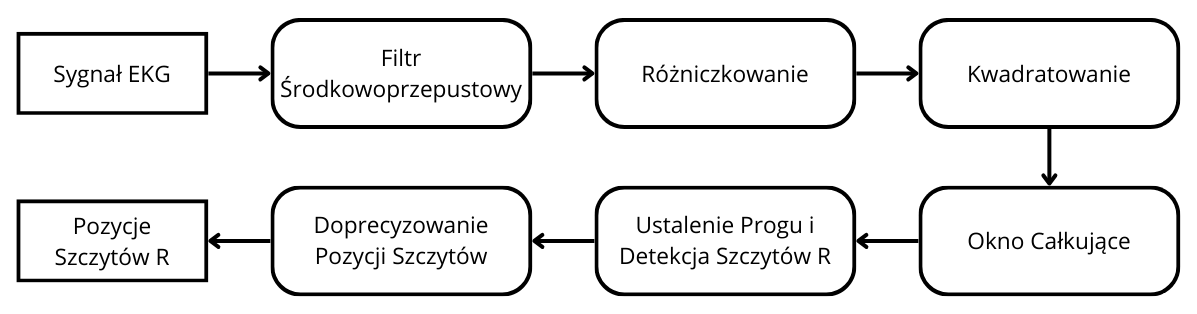
\includegraphics[scale=0.5]{Rysunki/Pan-Tomkins-scheme.png}
    \caption{Schemat algorytmu Pan-Tompkins z dodatkowym krokiem}
    \label{fig/PanTompkinsFlowChart}
\end{figure}

% \subsection{Filtracja �rodkowoprzepustowa}
Filtracja �rodkowoprzepustowa ma na celu usuni�cie zak��ce� wyst�puj�cych w
sygnale, co za tym idzie zwi�kszenie stosunku sygna�u do szumu
\cite{Fariha-PanTompkins}. Algorytm Pan-Tompkins standardowo wykorzystuje
filtracj� w pa�mie 5�15 Hz \cite{Fariha-PanTompkins}. Jednak na wczesnym etapie
realizacji projektu zaobserwowano, �e zastosowanie szerszego pasma filtracji
5-18 Hz, zaproponowanego w pracy \cite{Khan-PanTompkins++}, prowadzi�o do nieco
lepszych rezultat�w.

\begin{figure}[ht]
    \centering
    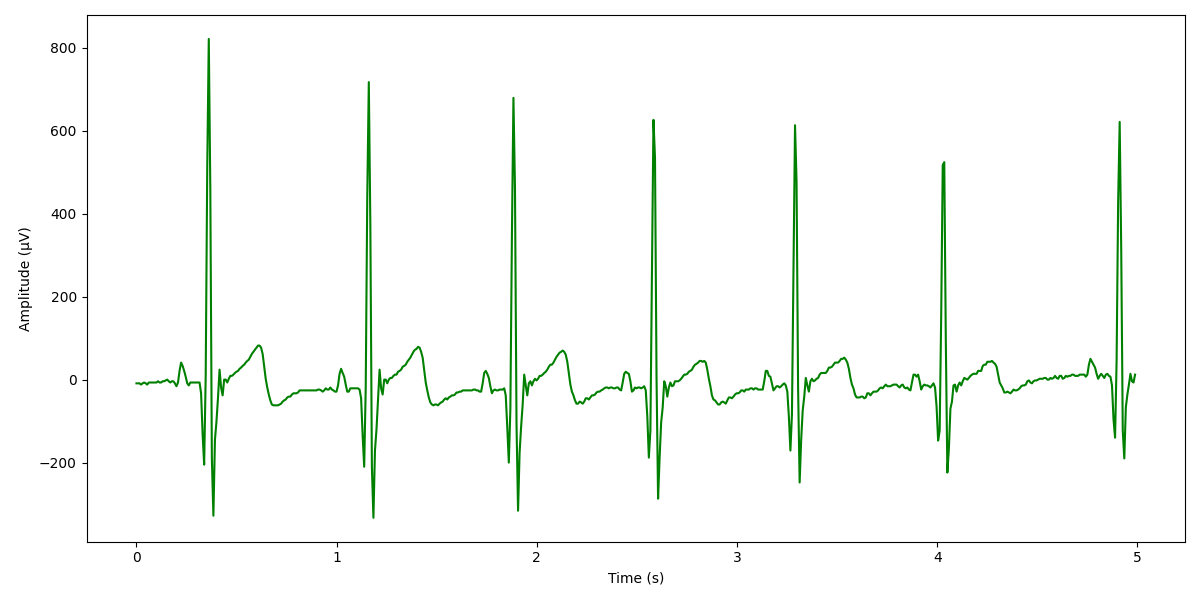
\includegraphics[scale=0.25]{Rysunki/Pan Tompkins_raw.png}
    \caption{Fragment surowego sygna�u EKG z czujnika Polar H10}
    \label{fig/PanTompkinsRaw}
\end{figure}

\begin{figure}[ht]
    \centering
    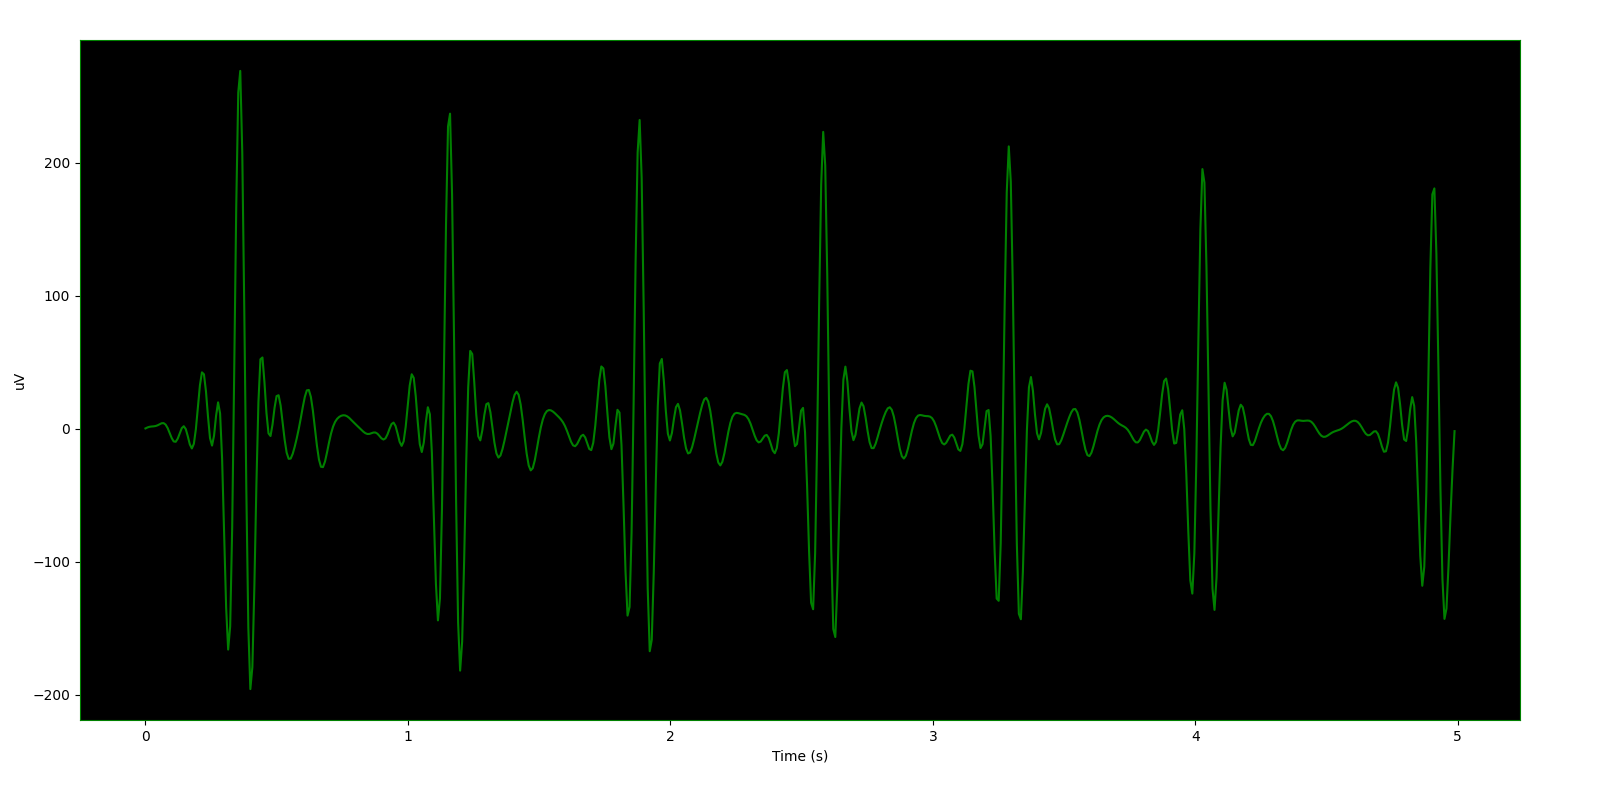
\includegraphics[scale=0.25]{Rysunki/Pan_tomkins_5_15.png}
    \caption{Fragment przefiltrowanego sygna�u EKG z czujnika Polar H10}
    \label{fig/PanTompkinsFiltered}
\end{figure}

% \subsection{R�niczkowanie}
Po wst�pnym przefiltrowaniu sygna� EKG jest poddawany r�niczkowaniu, co ma na
celu uwypuklenie szybko�ci zmian w sygnale, co pozwala na lepsze wyr�nienie
charakterystycznych punkt�w, takich jak szczyty R. W procesie wyznaczania
pochodnej nisko-cz�stotliwo�ciowe sk�adowe sygna�u s� t�umione, a
gwa�towniejsze zmiany uwypuklane, skutkuje to m. in. st�umieniem fal P i T oraz
wzmocnieniem bardziej stromych zbocz w kompleksie QRS
\cite{Fariha-PanTompkins}.\\

\begin{figure}[ht]
    \centering
    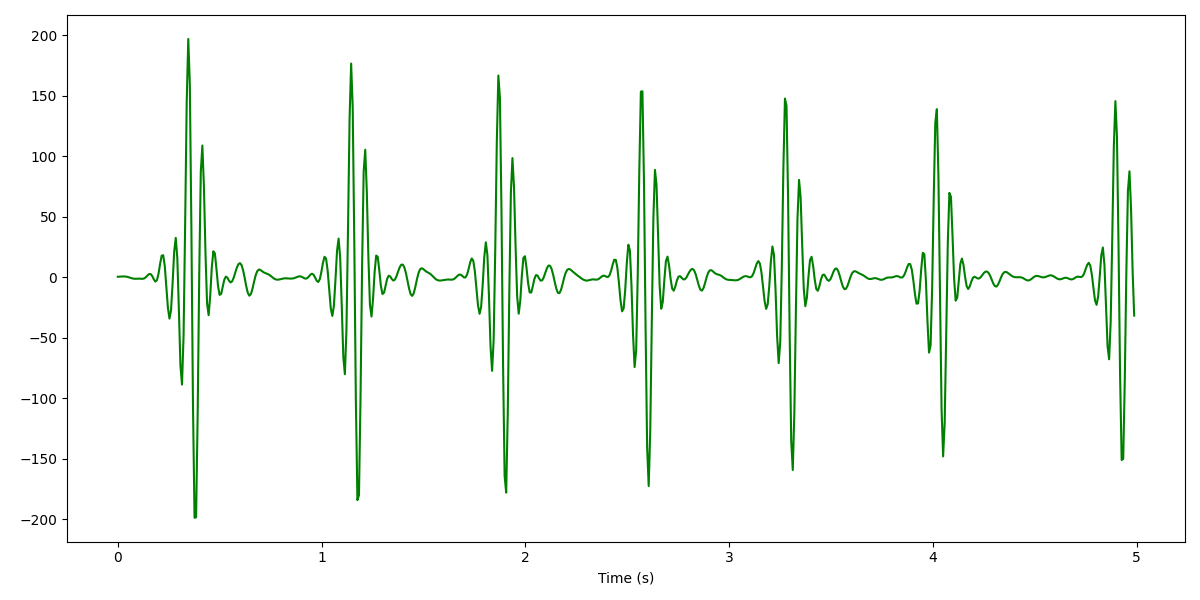
\includegraphics[scale=0.25]{Rysunki/PanTompkins_derivative.png}
    \caption{Fragment sygna�u EKG z czujnika Polar H10 po r�niczkowaniu}
    \label{fig/PanTompkinsDerivative}
\end{figure}

% \subsection{Kwadratowanie}
Kwadratowanie jest kolejnym etapem, w kt�rym sygna� uzyskany w poprzednim kroku
zostaje podniesiony do kwadratu. Dzi�ki temu wszystkie warto�ci sygna�u staj�
si� dodatnie, a fragmenty odpowiadaj�ce kompleksowi QRS staj� si� bardziej
widoczne. Dodatkowo, proces kwadratowania wyra�niej uwypukla r�nic� mi�dzy
kompleksem QRS a fal� T, co pozwala na ich lepsze rozr�nienie i redukuje
ryzyko fa�szywych wykry� szczyt�w R \cite{Fariha-PanTompkins}. \\

\begin{figure}[ht]
    \centering
    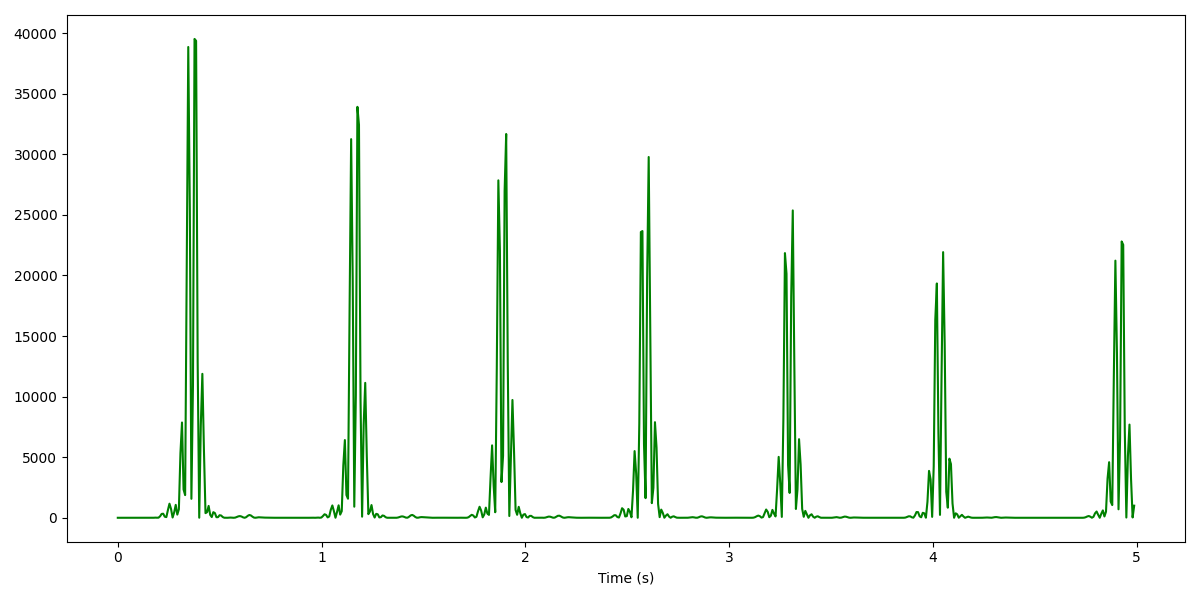
\includegraphics[scale=0.25]{Rysunki/Pan_tomkins_squared.png}
    \caption{Fragment sygna�u EKG z czujnika Polar H10 po kwadratowaniu}
    \label{fig/PanTompkinsSquared}
\end{figure}

% \subsection{Okno ca�kuj�ce}
Okno ca�kuj�ce ma na celu wyg�adzenie i u�rednienie sygna�u w okre�lonym
przedziale, oknie czasowym. Proces ten polega na obliczaniu sumy warto�ci
pr�bek sygna�u w ramach przesuwaj�cego sie okna, co prowadzi do uzyskania
bardziej sp�jnego i wyg�adzonego sygna�u wyj�ciowego. W ten spos�b uwypuklane
s� d�ugotrwa�e trendy i zmiany sygna�u, co znacznie u�atwia wykrywanie
charakterystycznych za�amk�w QRS. Okno ca�kuj�ce pomaga r�wnie� w eliminacji
mniejszych zak��ce�, kt�re mog�yby powodowa� fa�szywe wykrycia szczyt�w,
zwi�kszaj�c precyzj� i wiarygodno�� procesu detekcji. Dzi�ki zastosowaniu tego
etapu mo�liwe jest uzyskanie lepszej separacji szczyt�w R od pozosta�ych
element�w sygna�u. Dla danych pochodz�cych z czujnika Polar H10 zastosowano
okno o szeroko�ci 150 ms \cite{Fariha-PanTompkins}, co przek�ada�o si� na oko�o
20 pr�bek, bior�c pod uwag� cz�stotliwo�� pr�bkowania czujnika: 130 Hz.

\begin{figure}[ht]
    \centering
    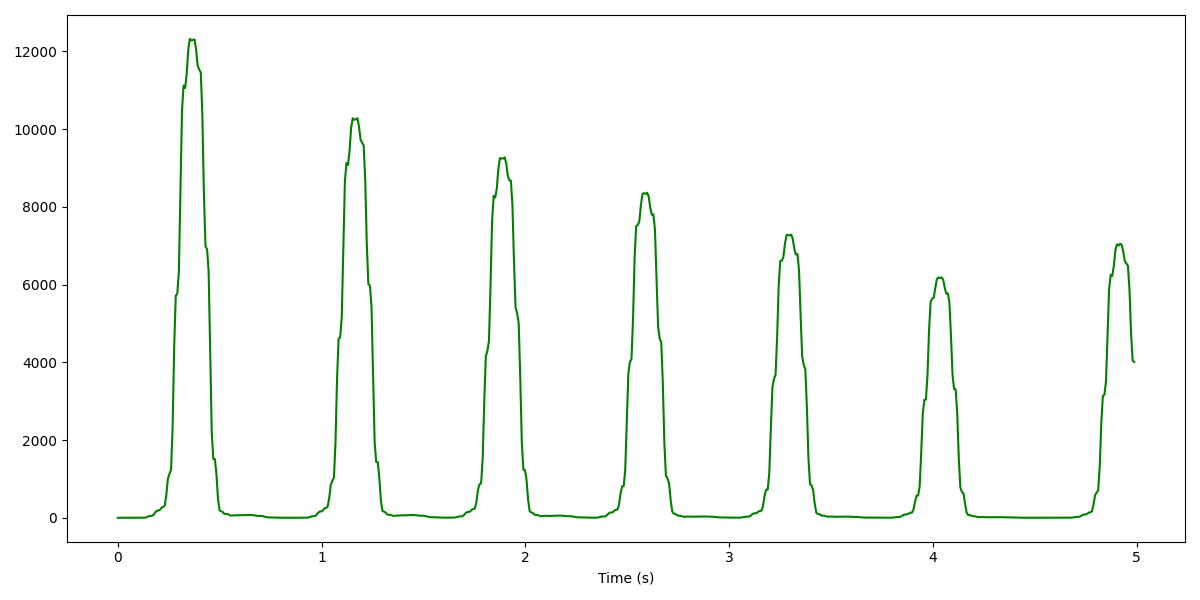
\includegraphics[scale=0.25]{Rysunki/Pan_tomkins_integrated.png}
    \caption{Fragment sygna�u EKG z czujnika Polar H10 po oknie ca�kuj�cym}
    \label{fig/Pan_tomkins_MWI}
\end{figure}

% \subsection{Ustalenie progu i detekcja szczyt�w R}
Ustalenie progu ma na celu detekcj� szczyt�w R, przy jednoczesnej minimalizacji
fa�szywych wykry�. W tym celu ustalany jest pr�g na bazie kt�rego podejmowana
jest decyzja. Pr�g ten mo�e by� warto�ci� sta�� lub by� dynamicznie
dostosowywany, aby uwzgl�dni� zmiany amplitudy w r�nych odcinkach sygna�u.
Podczas oznaczania danych pochodz�cych z czujnika Polar H10 zastosowano pr�g
obliczany jako �rednia warto�� sygna�u ca�kowanego powi�kszona o 0,6-krotno��
odchylenia standardowego tego sygna�u.\\

Podczas procesu detekcji warto�ci sygna�u por�wnywane s� z ustalonym progiem.
Gdy sygna� przekroczy warto�� progu, wst�pnie identyfikowany jest jako
potencjalny szczyt R. W celu minimalizacji fa�szywych wykry� stosuje si�
dodatkowe regu�y, takie jak minimalny odst�p czasowy pomi�dzy wykrytymi
szczytami. Podczas analizy danych pochodz�cych z czujnika Polar H10 zastosowano
odst�p wynosz�cy 400 ms.

\begin{figure}[ht]
    \centering
    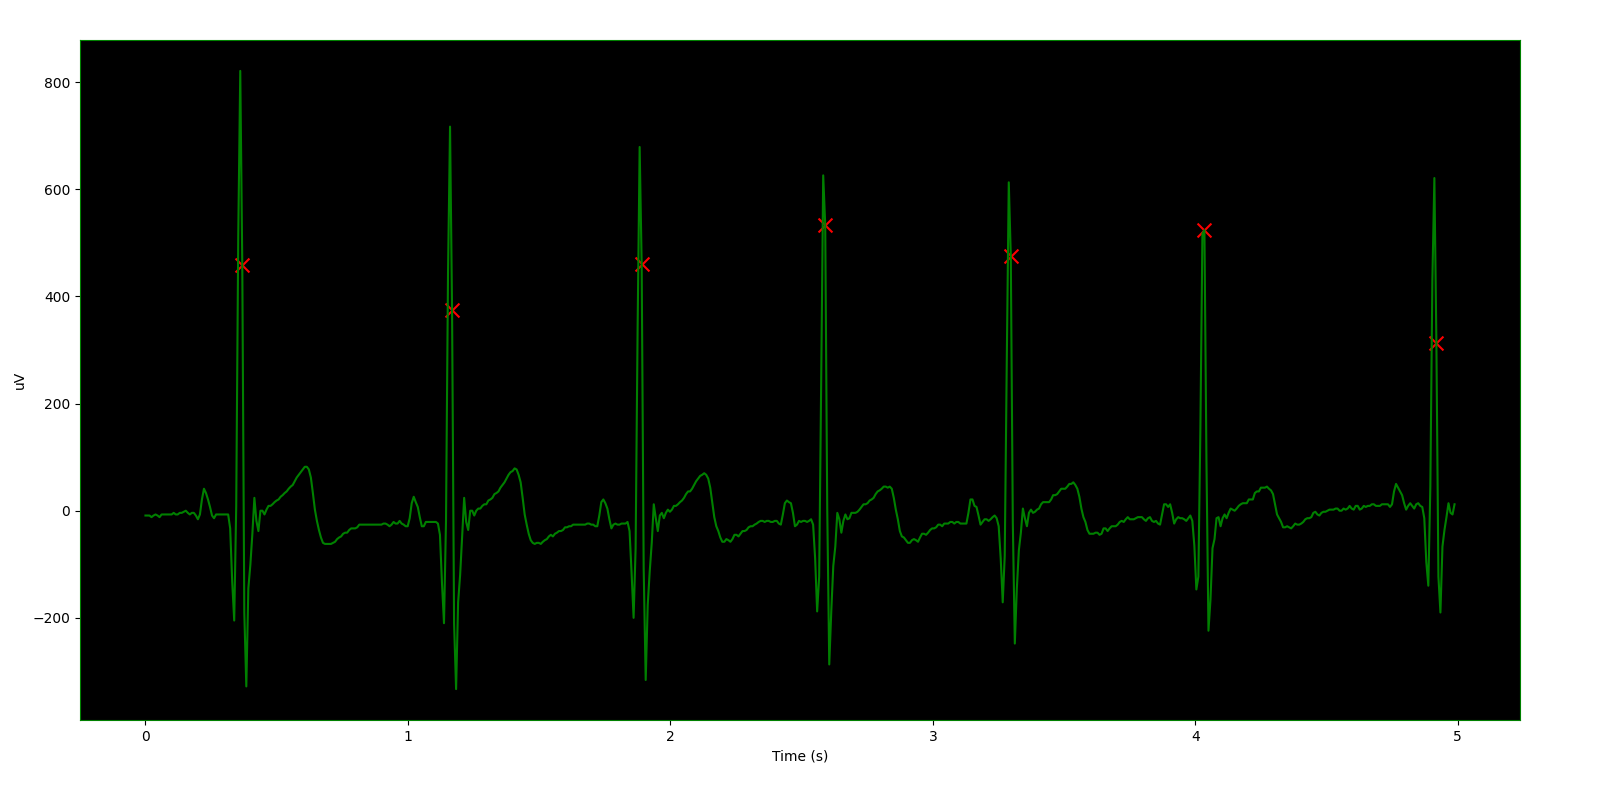
\includegraphics[scale=0.25]{Rysunki/Pan Tomkins without refining.png}
    \caption{Fragment sygna�u EKG z czujnika Polar H10 po wykryciu szczyt�w}
    \label{fig/Pan_tomkins_peaks}
\end{figure}

% \subsection{Doprecyzowanie pozycji szczyt�w}
W dodatkowym kroku przeanalizowano otoczenie wykrytych szczyt�w w pierwotnym
sygnale EKG w celu zwi�kszenia precyzji detekcji. Bez tej dodatkowej analizy
wykryte za�amki cz�sto by�y lekko przesuni�te wzgl�dem faktycznego maksimum
sygna�u. Dlatego dla ka�dego wykrytego punktu zbadano jego otoczenie i jako
szczyt oznaczono warto�� maksymaln� w tym zakresie. W przypadku danych
pochodz�cych z czujnika Polar H10 rozmiar okna, w kt�rym poszukiwano warto�ci
maksymalnej, zosta� ustalony na 10 pr�bek w obu kierunkach.\\

\begin{figure}[ht]
    \centering
    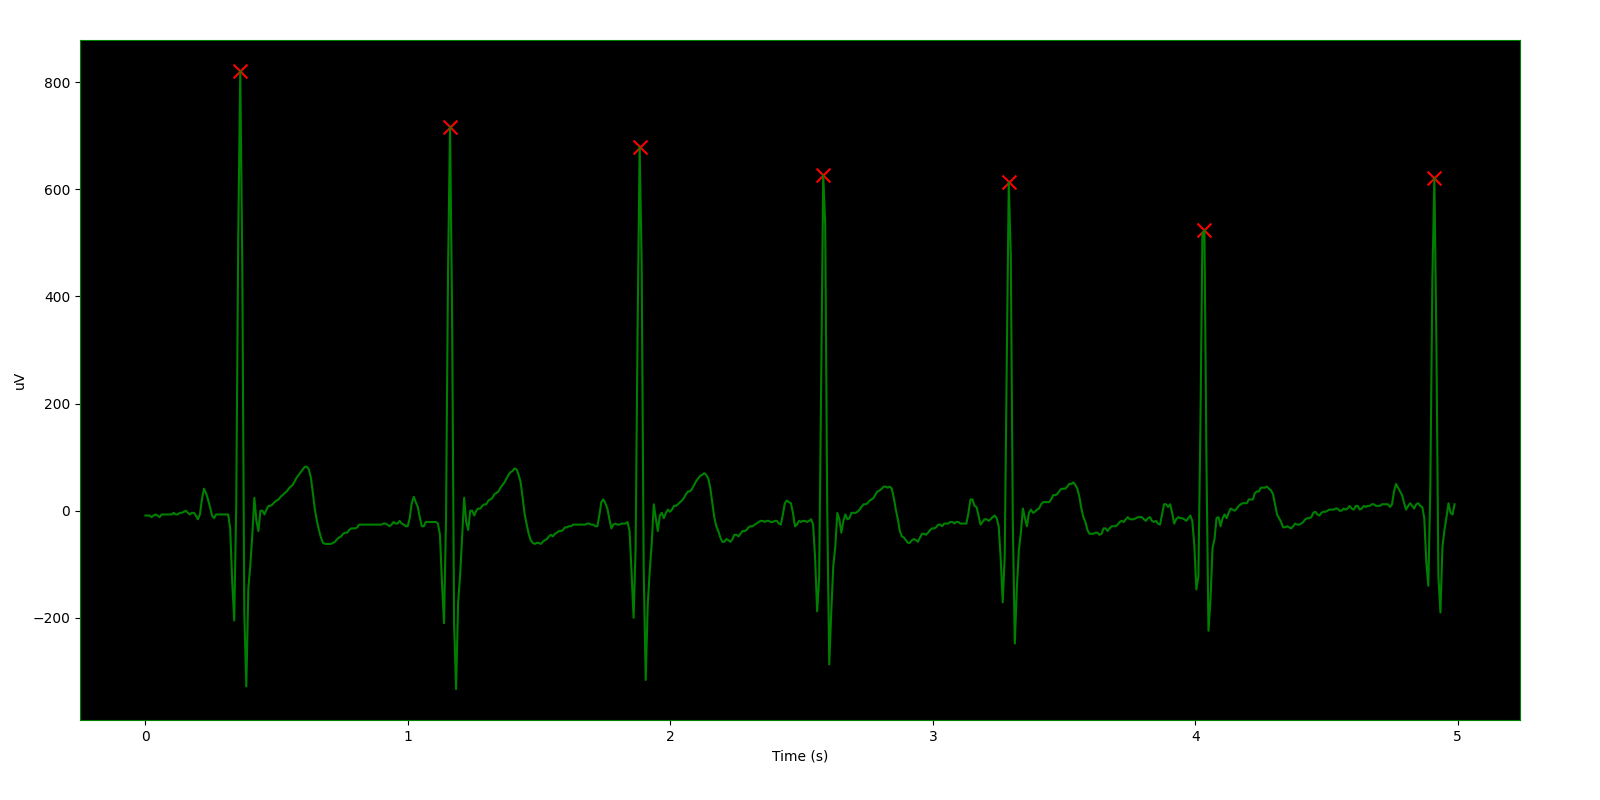
\includegraphics[scale=0.25]{Rysunki/Pan_tomkins_final.png}
    \caption{Fragment sygna�u EKG z czujnika Polar H10 po doprecyzowaniu pozycji szczyt�w}
    \label{fig/Pan_tomkins_refined_peaks}
\end{figure}

\subsection{Sie� UNet}

% Nast�pn� metoda wykorzystana do wyznaczenia pozycji sczyt�w R w niniejszej pracy jest sie�
% neuronowa oparta o architektur� 1D UNet, zaczerpni�ta z pracy
% \cite{MUzairZahid-UNET}. Schemat budowy sieci, wraz z blokiem postprocessingu i
% weryfikacji, przedstawiono na Rys. \ref{fig/UNet}, pochodz�cym z tej samej
% publikacji. Calo�� zosta�a zrealizowana przy u�yciu biblioteki TensorFlow, z
% wykorzystaniem jej wysokopoziomowego API o nazwie Keras
% \cite{TensorFlow-Keras}.

Kolejn� metod� wykorzystan� w niniejszej pracy do wyznaczenia pozycji za�amk�w
R jest sie� neuronowa oparta na architekturze 1D U-Net, zaczerpni�ta z pracy
\cite{MUzairZahid-UNET}.
% Schemat budowy sieci, uwzgl�dniaj�cy blok
% postprocessingu i weryfikacji, przedstawiono na rysunku \ref{fig/UNet}, kt�ry
% pochodzi z tej samej publikacji. 
Sie� opiera si� na modelu koder-dekoder, sk�adaj�cym si� z dw�ch g��wnych
element�w: �cie�ki koduj�cej i �cie�ki dekoduj�cej. Implementacja w projekcie
in�ynierskim bazuje na kodzie udost�pnionym przez autor�w, jednak zosta�a
zmodyfikowana i dostosowana do potrzeb projektu. Ca�o�� zrealizowano przy
u�yciu biblioteki TensorFlow oraz jej wysokopoziomowego API o nazwie Keras
\cite{TensorFlow-Keras}. Schemat budowy sieci, pochodz�cy z tej samej
publikacji, przedstawiono na Rys \ref{fig/UNet}

\begin{figure}[ht]
    \centering
    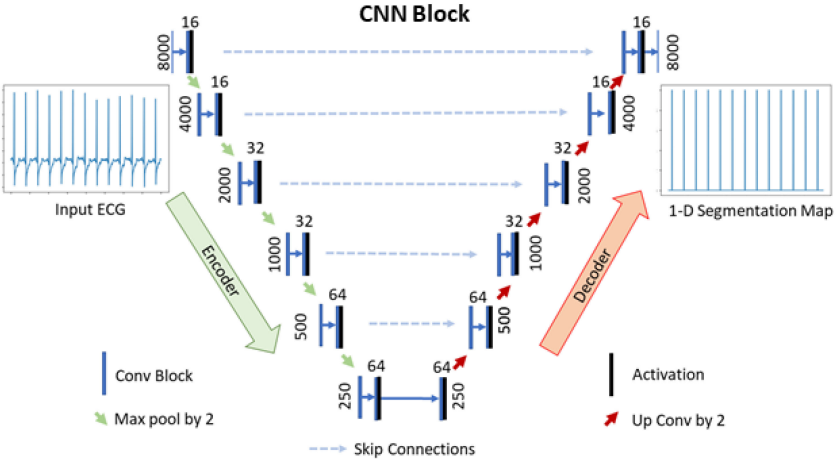
\includegraphics[scale=0.5]{Rysunki/U-net_small.png}
    \caption{Schemat sieci U-Net}
    \label{fig/UNet}
\end{figure}

% �cie�ka koduj�ca odpowiada za ekstrakcje istotnych cech sygna�u. �cie�ke koduj�c� z�o�ono z 6 warstw. Na ka�da warstw� tej �cie�ki sk�ada si� warstwa splotowa i funkcja aktywacji LeakyRELU. Warstwa splotowa dokonuje jednocze�nie operacji splotu i dwukrotnej redukcji wektora wej�ciowego, poprzez parametr stride, definiuj�cego rozmiar kroku przesuwania filtra. 

�cie�ka koduj�ca w modelu zosta�a zaprojektowana w celu ekstrakcji kluczowych cech sygna�u wej�ciowego oraz jego kontrolowanej redukcji. Sk�ada si� z sze�ciu warstw, z kt�rych ka�da realizuje przetwarzanie danych poprzez operacje splotu oraz funkcj� aktywacji LeakyReLU.

Ka�da warstwa wykorzystuje jednowymiarow� warstw� splotow� (Conv1D), kt�ra
wykonuje operacj� konwolucji na danych wej�ciowych, umo�liwiaj�c wyodr�bnienie
istotnych cech sygna�u. Warstwa ta jednocze�nie zmniejsza d�ugo�� wektora
wyj�ciowego o po�ow� dzi�ki zastosowaniu parametru stride=2, kt�ry definiuje
krok przesuwania filtra. Aby zachowa� pe�n� informacj� w ca�ym zakresie
sygna�u, zastosowano parametr padding='same'. Dzi�ki temu wyj�cie uwzgl�dnia
ca�� d�ugo�� wej�cia, niezale�nie od rozmiaru filtra, a brakuj�ce warto�ci s�
uzupe�niane zerami. Ostateczny rozmiar wyj�cia jest kontrolowany przez parametr
stride, kt�ry decyduje o stopniu redukcji danych. Liczba filtr�w oraz ich
rozmiar zmieniaj� si� co dwie warstwy i wynosz� odpowiednio: 16, 32, 64 dla
liczby filtr�w oraz 9, 6, 3 dla rozmiaru filtra.\\

�cie�ka dekoduj�ca odpowiada za rekonstrukcj� sygna�u wyj�ciowego na podstawie zakodowanych cech dostarczonych przez �cie�k� koduj�c�. Sk�ada si� z sze�ciu warstw transponowanych splot�w (Conv1DTranspose), kt�re realizuj� operacje odwrotne do warstw koduj�cych. Warstwy te zwi�kszaj� d�ugo�� wektora wyj�ciowego dwukrotnie dzi�ki zastosowaniu parametru stride=2, co pozwala na stopniowe przywracanie pierwotnego rozmiaru sygna�u wej�ciowego. Podobnie jak w �cie�ce koduj�cej, zastosowano parametr padding='same', aby zachowa� zgodno�� d�ugo�ci wyj�cia na ka�dym etapie rekonstrukcji. W pierwszej warstwie dekoduj�cej zastowsowano r�wnie� mechanizm dropout z prawdopodobienstwem 0.25, w celu zignorowania pewnej liczby neuron�w i poprawy generalizacji sieci. Ka�da warstwa dekoduj�ca wykorzystuje funkcj� aktywacji LeakyReLU, z wyj�tkiem ostatniej, gdzie zastosowano funkcj� sigmoid, co wprowadza nieliniowo�� do procesu dekodowania. Ostatnia wartstwa wykorzystuje wy��cznie jeden filtr, w celu wygenerowania jednego kana�u wyj�ciowego.
Wynikiem przetwarzania fragmentu sygna�u przez model jest jednowymiarowa mapa segmentacji, kt�ra przedstawia prawdopodobie�stwo ka�dej pr�bki sygna�u na bycie szczytem R.

Kazda z warstw modelu, z wyj�tkiem pierwszej, korzysta r�wnie� z normalizacji
wsadowej (BatchNormalization), co pozwala na stabilizacje oraz przyspieszenie
procesu uczenia poprzez standaryzacje danych.

W podanym modelu zastosowano po��czenia skip connections, kt�re umo�liwiaj�
po��czenie wyj�� z warstw koduj�cych z danymi przetwarzanymi w �cie�ce
dekoduj�cej. W trakcie przechodzenia sygna�u przez �cie�k� koduj�c�, wyj�cia z
ka�dej warstwy koduj�cej s� zapisywane na osobnej li�cie. W �cie�ce dekoduj�cej
te zapisane wyj�cia z warstw koduj�cych s� p�niej wykorzystywane do po��czenia
z aktualnymi danymi przetwarzanymi w dekoderze. Po��czenie to realizowane jest
za pomoc� operacji konkatenacji (Concatenate), kt�ra ��czy dwa zestawy danych �
wyj�cie z warstwy dekoduj�cej oraz odpowiadaj�ce mu wyj�cie z warstwy koduj�cej
� wzd�u� osi kana��w. Powoduje to, �e dekoder korzysta z bogatszego zestawu
informacji, zawieraj�cego zar�wno cechy szczeg�owe, jak i bardziej og�lne. To
po��czenie pozwala na dok�adniejsz� rekonstrukcj� sygna�u i unikni�cie utraty
szczeg��w w procesie kodowania.\\

Wynik uzyskany z modelu wymaga dodatkowego przetwarzania, aby precyzyjnie
zidentyfikowa� rzeczywiste za�amki R. Ca�y proces wykrywania tych szczyt�w, od
sygna�u do wynik�w, przebiega w nast�puj�cych etapach:
\begin{enumerate}
    \item Podzia� sygna�u na okna: Sygna� jest dzielony na nachodz�ce na siebie okna. W
          tej pracy zastosowano parametr stride r�wny 3/4 wielko�ci pojedynczego okna, co
          zapewnia cz�ciowe nak�adanie si� okien.
    \item Przetwarzanie przez model: Ka�de okno jest przepuszczane przez model, kt�ry
          generuje map� prawdopodobie�stw dla pr�bek w tym oknie.
    \item Scalanie wynik�w: Uzyskane wyniki z nak�adaj�cych si� okien s� ��czone i
          u�redniane, co redukuje b��dy na granicach okien i pozwala uzyska� jedn�,
          sp�jn� map� prawdopodobie�stw dla ca�ego sygna�u.
    \item Selekcja punkt�w: Na podstawie zdefiniowanego progu (w tym przypadku threshold
          = 0.5) wybierane s� punkty o wysokim prawdopodobie�stwie bycia szczytem R.
    \item Korekcja punkt�w: Wybrane punkty s� przesuwane w kierunku warto�ci, kt�ra jest
          najbardziej oddalona od �redniej wyg�adzonego sygna�u. Proces ten realizowany
          jest za pomoc� funkcji \emph{correct\textunderscore peaks} z modu�u
          \emph{wfdb.processing}
    \item Finalne rozpoznanie szczyt�w R: Je�li co najmniej pi�� punkt�w zostanie
          podci�gni�te do tego samego miejsca, punkt ten zostaje zaklasyfikowany jako
          szczyt R.
\end{enumerate}

\vspace{1em}
\begin{figure}[ht]
    \centering
    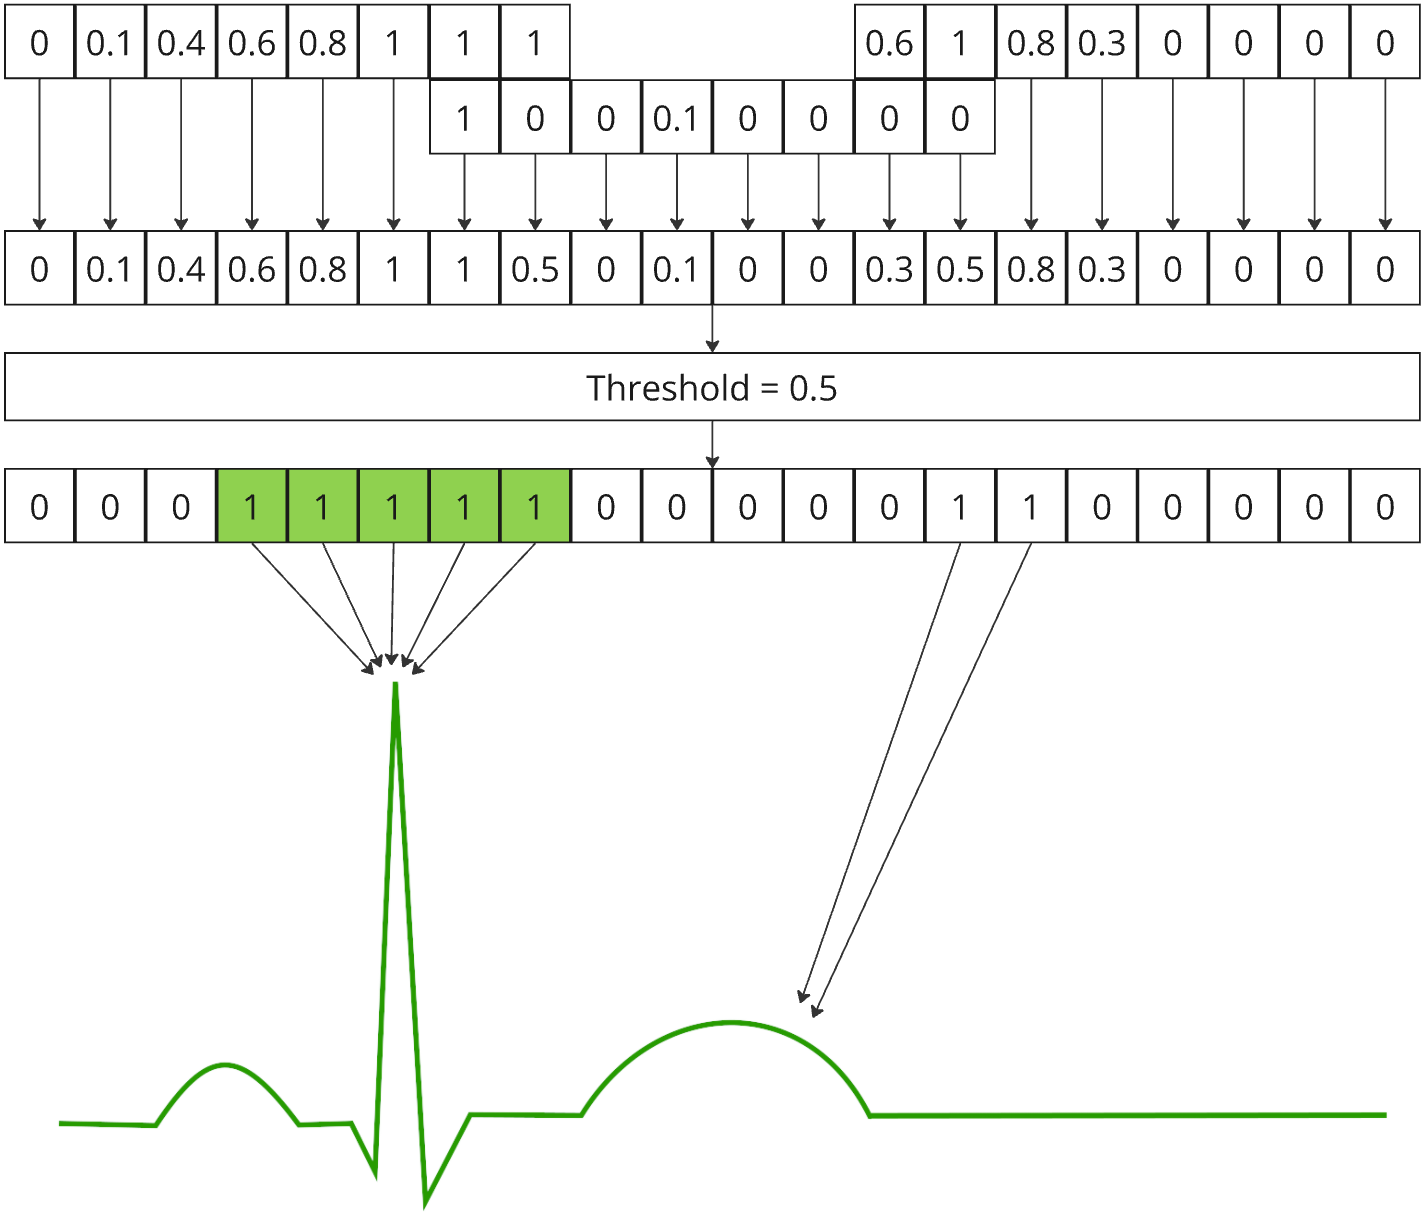
\includegraphics[scale=1]{Rysunki/unet-postprocess.png}
    \caption{Uproszczony schemat przetworzenia wynik�w sieci, od otrzymanych map segmentacji z sieci do rozpoznania szczytu}
    \label{fig/UNet-r-preak-identification}
\end{figure}

W ramach modyfikacji wzgl�dem pierwotnej implementacji zmieniono spos�b korekty
za�amk�w R � w pierwotnej wersji korekta by�a zawsze wykonywana do warto�ci
najwy�szej, natomiast wprowadzone zmiany pozwalaj� na korekt� do warto�ci
najbardziej oddalonej od �redniej. Udoskonalenie to umo�liwi�o poprawne
rozpoznawanie za�amk�w R nawet w przypadku odwr�cenia sygna�u EKG, na przyklad
z powodu zamiany polaryzacji elektrod. Metod� wykrywania szczyt�w obudowano w�asnym interfejsem,
kt�ry by� wspomniany w podsekcji \ref{subsec:wykrywacz} 

% W ramach modyfikacji wzgl�dem pierwotnej implementacji zmniejszono rozmiar okna
% (autorzy zalecali zakres od 5 do 20 sekund) do oko�o 1,5 sekundy, co umo�liwi�o
% zastosowanie algorytmu w czasie rzeczywistym. Ponadto zmieniono spos�b korekty
% za�amk�w R � w pierwotnej wersji korekta by�a zawsze wykonywana do warto�ci
% najwy�szej, natomiast wprowadzone zmiany pozwalaj� na korekt� do warto�ci
% najbardziej oddalonej od �redniej. Udoskonalenie to umo�liwi�o poprawne
% rozpoznawanie za�amk�w R nawet w przypadku odwr�cenia sygna�u EKG, na przyklad
% z powodu zamiany polaryzacji elektrod. Metod� obudowano w�asnym interfejsem,
% kt�ry by� wspomniany w podsekcji \ref{subsec:wykrywacz} 
\FloatBarrier
\section{Modele neuronowe do wyznaczania miar HRV}
\subsection{Model oparty o interwa�y RR}\label{rr-based}
% \subsection{Model do wyznaczania miar HRV na bazie interwa��w RR}
W trakcie prac nad modelem end-to-end opracowano model po�redni, kt�ry
przewiduje miary HRV na podstawie interwa��w RR. Pocz�tkowo planowano jego
intergracje z modelem UNet w jedn� sie� typu end-to-end, jednak ostatecznie
zrezygnowano z tego podej�cia. Model end-to-end zosta� stworzony jako
bezpo�rednie rozwini�cie tego modelu. Do implementacji modelu wykorzystano
wysokopoziomowe API biblioteki \emph{tensorflow} o nazwie \emph{Keras}
\cite{TensorFlow-Keras}. Schemat modelu po�redniego przedstawiono na Rys.
\ref{fig/rr_siec}.

Model oparto o kaskade trzech blok�w przetwarzania, z kt�rych ka�dy zawiera
jednowymiarowa warstw� splotow� (Conv1D), normalizacje wsadow�
(BatchNormalization) oraz operacje maksymalnego pr�bkowania (MaxPooling1D).
Warstwy splotowe wykorzystuj� funkcj� aktywacji ReLU i parametr padding=same,
kt�ry zachowuje rozmiar wyj�cia taki sam jak wej�cia. Rozmiary filtr�w w
warstwach splotowych wynosz� odpowiednio 7, 5 i 3, a ich ilo�� to 64, 128 i
256. Maksymalne pr�bkowanie zmniejsza dwukrotnie rozmiar danych na ko�cu
ka�dego z blok�w poprzez zastosowanie parametru pool\_size=2, oznaczaj�cego, �e
dla ka�dej pary s�siaduj�cych pr�bek wybierana jest warto�� maksymalna.

Po przej�ciu przez pierwsze bloki przetwarzaj�ce wyniki trafiaj� do warstwy
rekurencyjnej LSTM (Long Short-Term Memory), kt�ra zawiera 128 jednostek.
Wartswa ta przetwarza dane sekwencyjne, ucz�c si� wzorc�w czasowych w sygnale.
Na wyj�ciu warstwy LSTM zastosowano warstw� dropout na poziomie 30\%, co
oznacza, �e w trakcie treningu 30\% neuron�w jest losowo dezaktywowanych.
Zapobiega to przeuczeniu modelu oraz poprawia jego zdolno�ci generalizacyjne.

Na ko�cu model zawiera ostatni� warstw� gest�, kt�rej liczba neuron�w odpowiada
liczbie przewidywanych przez model warto�ci, na przyk�ad w przypadku
przewidywania SDNN i RMSSD rozmiar ten wynosi dwa. Warstwa ta wykorzystuje
liniowa funkcje aktywacji, co pozwala na generowanie ci�g�ych warto�ci
wyjsciowych, zgodnych ze skala przewidywanych miar.

\begin{figure}[ht]
    \centering
    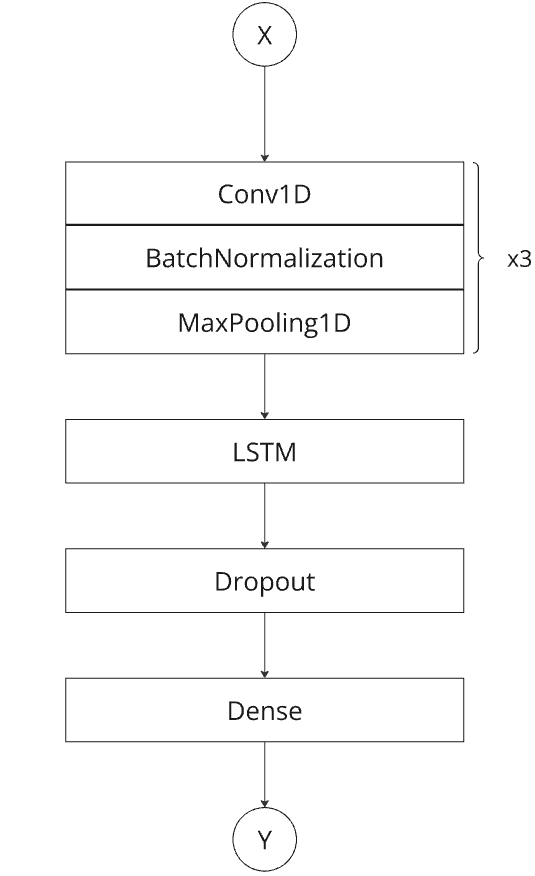
\includegraphics[scale=1.5]{Rysunki/RR_siec.png}
    \caption{Schemat modelu wyznaczaj�cego miary HRV na podstawie interwa��w RR}
    \label{fig/rr_siec}
\end{figure}

% \subsection{Model end-to-end do wyznaczania miar HRV}\label{siec-end-to-end}\
\FloatBarrier
\subsection{Model end-to-end}\label{siec-end-to-end}
W ramach pracy opracowano model sieci neuronowej typu end-to-end, b�dacy
rozwojow� wersj� prostego modelu opartego o interwa�y RR, opisanego w
podrozdziale \ref{rr-based}. Jego przeznaczeniem jest przewidywanie parametr�w
HRV na podstawie surowego sygna�u EKG. Do jego implementacji wykorzystano
wysokopoziomowe API biblioteki \emph{tensorflow} o nazwie \emph{Keras}
\cite{TensorFlow-Keras}. Schemat architektury sieci przedstawiono na Rys.
\ref{fig/end-to-end}

\begin{figure}[!ht]
    \centering
    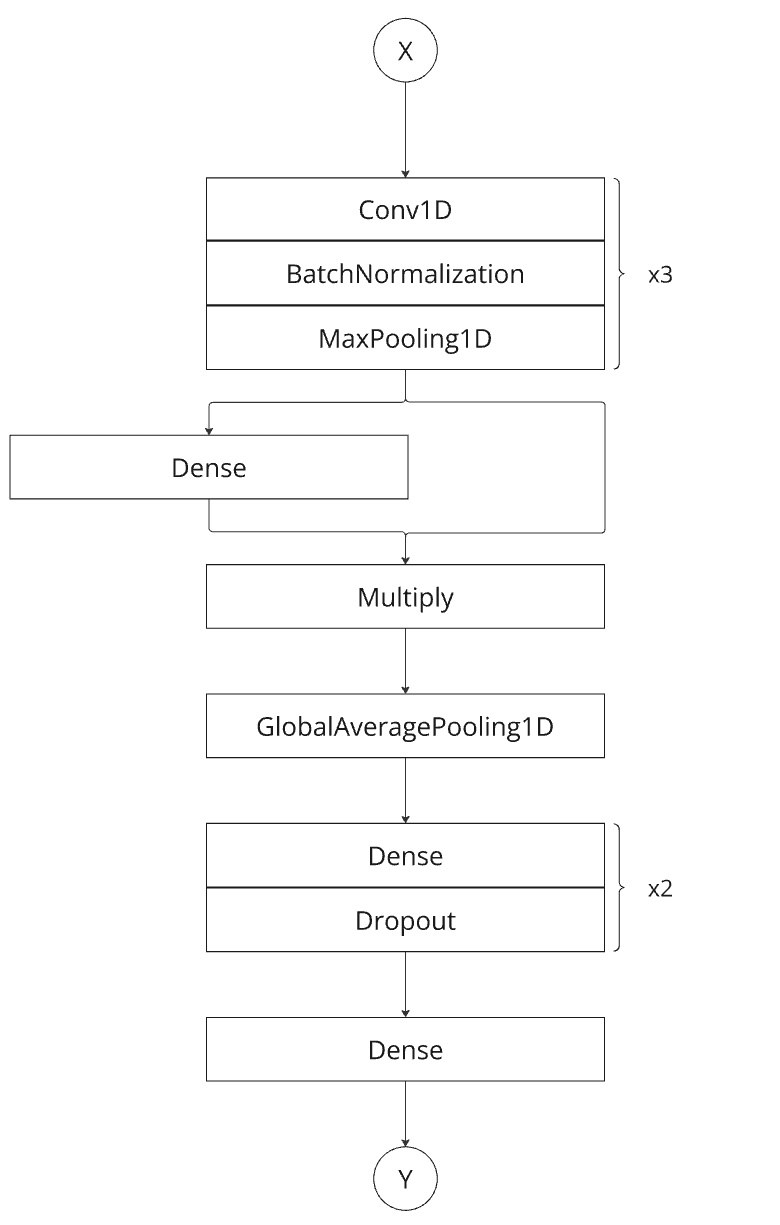
\includegraphics[scale=1.5]{Rysunki/end-to-end.png}
    \caption{Schemat modelu end-to-end do wyznaczania miar HRV}
    \label{fig/end-to-end}
\end{figure}

Model u�ywa takiej samej kombinacji blok�w przetwarzaj�cych co pierwowz�r,
jednak ze zmodyfikowanymi parametrami. Rozmiary j�der w warstwach
konwolucyjnych wynosz� kolejno 15, 11 i 9, a ich ilo�� zosta�a zmniejszona do
32, 64, oraz 128. Dodatkowo zmieniono parametr maksymalnego pr�bkowania: w
pierwszych dw�ch warstwach zastosowano pi�ciokrotn� redukcj� wymiaru, a w
trzeciej warstwie czterokrotn�.

Po przej�ciu przez te trzy bloki, dane trafiaj� do warstwy uwagi,
zaimplementowanej przy u�yciu warstwy g�stej (Dense) z funkcj� aktywacji
sigmoid. Wynik tej warstwy jest przemna�any z wynikiem ostatniego bloku
przetwarzaj�cego. Nast�pnie dane s� globalnie u�redniane
(GlobalAveragePooling1D), co redukuje je do wektora reprezentuj�cego �rednie
warto�ci filtr�w wzd�u� ca�ego sygna�u.

Po operacji u�redniania dane przechodz� przez dwie warstwy g�ste, kt�rych
rozmiary wynosz� 128 i 64. Po ka�dej z tych warstw zastosowano mechanizm
losowego odrzucania neuron�w (dropout), odpowiednio na poziomie 40\% i 30\%.
Zapobiega to przeuczeniu modelu oraz wspiera jego generalizacje.

Ostatnia warstwa modelu pozosta�a niezmieniona w stosunku do pierwowzoru. Jest
to g�sta warstwa, kt�rej liczba neuron�w odpowiada liczbie przewidywanych
warto�ci. Na przyk�ad, przy prognozowaniu SDNN i RMSSD, warstwa ta zawiera dwa
neurony. Wykorzystuje ona liniow� funkcj� aktywacji, co umo�liwia modelowi
zwracanie ci�g�ych warto�ci wyj�ciowych, zgodnych z zakresem przewidywanych
parametr�w.

\FloatBarrier

% W ramach pracy opracowano model sieci neuronowej typu end-to-end, b�dacy
% rozwojow� wersj� prostego modelu opartego o interwa�y RR z kt�rego
% przeznaczeniem jest przewidywanie parametr�w HRV na podstawie surowego sygna�u
% EKG. Do implementacji sieci wykorzystano wysokopoziomowe API biblioteki
% \emph{tensorflow} o nazwie \emph{Keras} \cite{TensorFlow-Keras}. Schemat
% architektury sieci przedstawiono na Rys. \ref{fig/end-to-end}

% \begin{figure}[ht]
%     \centering
%     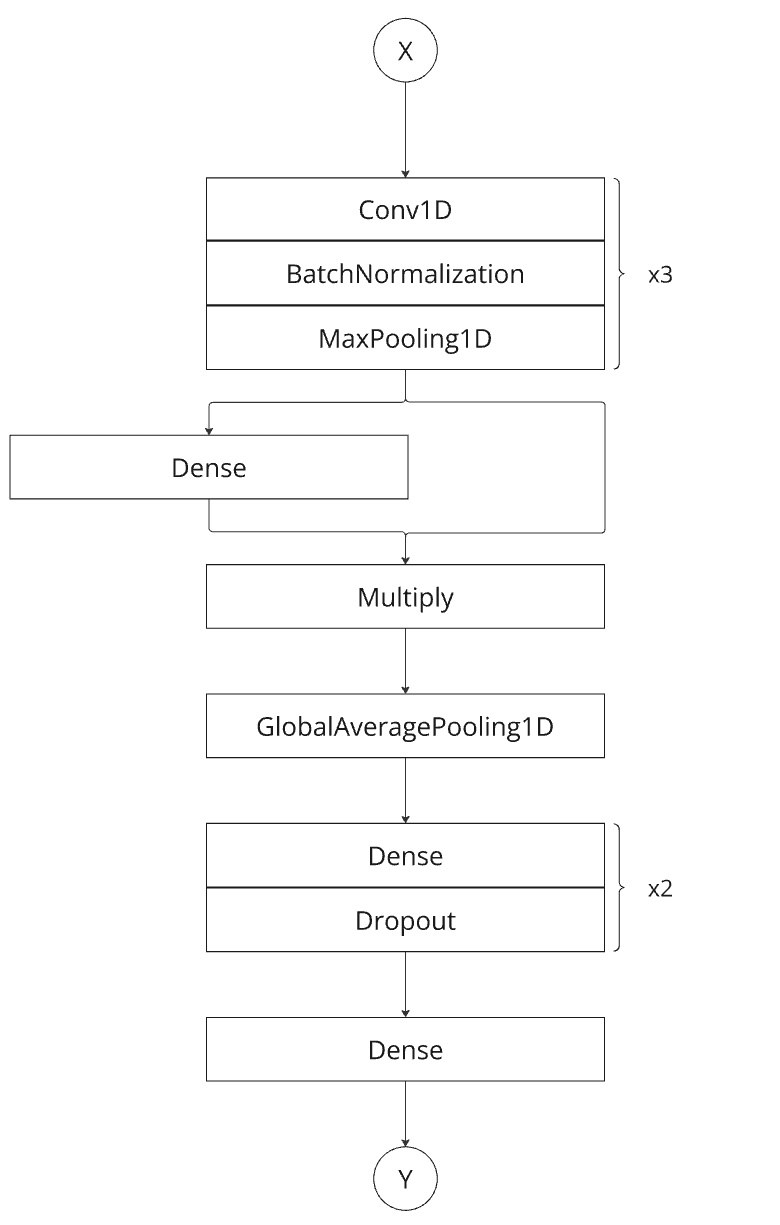
\includegraphics[scale=1.5]{Rysunki/end-to-end.png}
%     \caption{Schemat sieci end-to-end do wyznaczania miar HRV}
%     \label{fig/end-to-end}
% \end{figure}

% Model oparto o kaskade trzech blok�w przetwarzania, z kt�rych ka�dy zawiera
% jednowymiarowa warstw� splotow� (Conv1D), normalizacje wsadow�
% (BatchNormalization) oraz operacje maksymalnego pr�bkowania (MaxPooling1D).
% Warstwy splotowe wykorzystuj� funkcj� aktywacji ReLU i parametr padding=same,
% kt�ry zachowuje rozmiar wyj�cia taki sam jak wej�cia. Rozmiary filtr�w w
% warstwach splotowych wynosz� odpowiednio 15, 11 i 9, a ich ilo�� to 32, 64 i
% 128. Maksymalne pr�bkowanie zmniejsza rozmiar danych na koniec z ka�dego z
% blok�w, pieciokrotnie w przypadku pierwszych dw�ch oraz czterokrotnie w wypadku
% trzeciego.

% Po przej�ciu przez te trzy bloki, dane trafiaj� do warstwy uwagi,
% zaimplementowanej przy u�yciu warstwy g�stej (Dense) z funkcj� aktywacji
% sigmoid. Wynik tej warstwy jest przemna�any z wynikiem ostatniego bloku
% przetwarzaj�cego. Nast�pnie dane s� globalnie u�redniane
% (GlobalAveragePooling1D), co redukuje je do wektora reprezentuj�cego �rednie
% warto�ci filtr�w wzd�u� ca�ego sygna�u.

% Po operacji u�redniania dane przechodz� przez dwie warstwy g�ste, kt�rych
% rozmiary wynosz� 128 i 64. Po ka�dej z tych warstw zastosowano mechanizm
% losowego odrzucania neuron�w (dropout), odpowiednio na poziomie 40\% i 30\%.
% Zapobiega to przeuczeniu modelu oraz wspiera jego generalizacje.

% Na ko�cu model zawiera ostatni� warstw� gest�, kt�rej liczba neuron�w odpowiada
% liczbie przewidywanych przez model warto�ci, na przyk�ad w przypadku
% przewidywania SDNN i RMSSD rozmiar ten wynosi dwa. Warstwa ta wykorzystuje
% liniowa funkcje aktywacji.


\section{Metody uczenia maszynowego do analizy EKG}

\subsection{Rozpoznawanie arytmii}
ZROBI� JAKIS WST�P, ABY NIE DENERWOWAC PIOTRA.

Do rozpoznawania arytmii wykorzystuje si� szeroki zakres metod uczenia
maszynowego, obejmuj�cych zar�wno klasyczne podej�cia uczenia nadzorowanego,
jak i techniki uczenia nienadzorowanego. W�r�d klasycznych algorytm�w
nadzorowanych popularne s� SVM (Support Vector Machines), KNN (K-Nearest
Neighbors), klasyfikatory Bayesowskie, drzewa decyzyjne oraz lasy losowe.
Metody uczenia nienadzorowanego r�wnie� odgrywaj� istotn� rol�, wspieraj�c
proces eksploracji danych i in�ynierii cech, co mo�e znacz�co poprawi�
skuteczno�� modeli klasyfikacyjnych. W tym zakresie stosuje si� algorytmy takie
jak K-means, fuzzy c-means clustering, grupowanie hierarchiczne oraz Gaussian
Mixture Models. Ponadto coraz cz�ciej wykorzystuje si� g��bokie sieci
neuronowe, niewymagaj�ce w tym splotowe sieci neuronowe (CNN) oraz sieci LSTM
(Long Short-Term Memory) \cite{Kavya-shockableArthytmiaDetection}.

Ribeiro i wsp�autorzy \cite{ribeiro2020automatic} opracowali g��bok� sie�
neuronow� (DNN) do automatycznej klasyfikacji nieprawid�owo�ci w kr�tkotrwa�ych
(7-10 s), 12-odprowadzeniowych zapisach EKG. Algorytm zosta� wytrenowany na
zbiorze danych obejmuj�cym ponad 2,3 miliona zapis�w EKG. Architektura DNN
opiera�a si� na sieci rezydualnej przystosowanej do analizy sygna��w
jednowymiarowych, z warstwami konwolucyjnymi i po��czeniami skip dla
zwi�kszenia efektywno�ci treningu.

DNN zosta�a wytrenowana do wykrywania sze�ciu nieprawid�owo�ci: bloku
przedsionkowo-komorowego I stopnia, bloku prawej odnogi p�czka Hisa, bloku
lewej odnogi p�czka Hisa, bradykardii zatokowej, migotania przedsionk�w oraz
tachykardii zatokowej. Model osi�gn�� wysokie wyniki F1 (powy�ej 80\%) oraz
specyficzno�� (>99\%) dla ka�dej z klas, dor�wnuj�c lub przewy�szaj�c wydajno��
rezydent�w kardiologii i student�w medycyny.

Praca pokazuje potencja� DNN do nauki end-to-end, gdzie klasyfikacja odbywa si�
bezpo�rednio na podstawie surowych sygna��w EKG, bez konieczno�ci r�cznego
wyodr�bniania cech. Podkre�lono r�wnie� znaczenie du�ych, odpowiednio
oznaczonych zbior�w danych dla trenowania modeli oraz korzy�ci wynikaj�ce z
zastosowania g��bokiego uczenia w dok�adnej i skalowalnej interpretacji EKG w
praktyce klinicznej, zw�aszcza na obszarach z ograniczonym dost�pem do
specjalist�w. \\

Metod� klasyfikacji, nie opart� o sieci neuronowe przedstawiono w publikacji
\cite{Morteza-RandomForest}. Autorzy zaproponowali hybrydowy algorytm,
umo�liwiaj�cy przypisanie sygna�u do jednej z czterech klas: migotania
przedsionk�w (AF), normalnego rytmu zatokowego, innych rytm�w lub sygna��w zbyt
zak��conych do analizy. Proces ten opiera� si� na wykorzystaniu klasyfikatora
opartego o las losowy (Random Forest) zar�wno do selekcji cech, jak i do
finalnej klasyfikacji, co pozwoli�o na efektywne przetwarzanie i analiz� du�ej
liczby parametr�w.

W pocz�tkowej fazie sygna� EKG by� poddawany wst�pnemu przetworzeniu,
obejmuj�cego odszumianie i usuni�cie przesuni�cia bazowego. Nast�pnie
wyodr�bniono 491 cech opisuj�cych w�a�ciwo�ci sygna�u w domenach czasowej,
cz�stotliwo�ciowej, czasowo-cz�stotliwo�ciowej oraz przestrzeni fazowej.
Kolejnym etapem by�o wy�onienie najistotniejszych cech, kt�r� zosta�o
przeprowadzone za pomoc� Random Forest, na podstawie oceny ich wp�ywu na
zmniejszanie entropii w modelu. W ten spos�b uzyskano zbi�r 150 najbardziej
znacz�cych cech.

Ostateczna klasyfikacja odbywa�a si� r�wnie� za pomoc� Random Forest z 500
drzewami decyzyjnymi, z wykorzystaniem techniki baggingu oraz losowego wyboru
cech w w�z�ach, co zwi�ksza�o odporno�� na przeuczenie i poprawia�o stabilno��
predykcji. Algorytm osi�gn�� skuteczno�� 82,6\% na niezale�nym zbiorze
testowym, co zapewni�o mu ex aequo pierwsze miejsce w PhysioNet/Computing in
Cardiology Challenge 2017
\cite{Morteza-RandomForest}\cite{PhysioNet-Challange2017}.

\subsection{Wykrywanie sczyt�w R}
Wykrywanie szczyt�w R w sygnale EKG to kluczowy etap analizy, na podstawie
kt�rego obliczane s� istotne parametry pracy serca. Tradycyjne metody, takie
jak algorytm Pan-Tompkins, mimo swojej popularno�ci, cz�sto okazuj� si� podatne
na szumy i zak��cenia w sygnale, co ogranicza ich skuteczno�� w trudnych
warunkach. W odpowiedzi na te wyzwania coraz cz�ciej stosuje si� metody
uczenia maszynowego, takie jak splotowe sieci neuronowe (CNN) czy sieci LSTM
(Long Short-Term Memory), kt�re s� bardziej odporne na zak��cenia i lepiej
radz� sobie z analiz� z�o�onych wzorc�w sygna�u.

Przyk�ad zastosowania sieci LSTM w detekcji szczyt�w R przedstawiono w pracy
\cite{JUHO-LSTM}. Zaprezentowany model sk�ada� si� z dw�ch warstw
dwukierunkowych LSTM, kt�re wykorzystywa�y tangens hiperboliczny jako funkcje
aktywacji oraz warstwy g�stej z funkcj� sigmoid, generuj�c� prawdopodobie�stwo,
�e dany punkt w czasie to szczyt R. Do trenowania wykorzystano zbi�r danych
MIT-BIH Arrhythmia Database oraz MIT-BIH Noise Stress Test Database,
rozszerzaj�c zbi�r danych poprzez dodawanie realistycznych zak��ce�, takich jak
dryf linii bazowej czy artefakty mi�niowe. Model by� trenowany z u�yciem
optymalizatora Adam i funkcji strat binarnej entropii krzy�owej, na ponad 1,5
miliona przyk�ad�w.

Po odpowiednim odfiltrowaniu punkt�w o niskim prawdopodobie�swie, podej�cie
LSTM osi�gn�o wysokie wyniki, osi�gaj�c wyniik F1 na poziomie znacznie powy�ej
0.90, nawet przy niskim stosunku sygna�u do szumu (SNR 0.1). Zaproponowane
rozwi�zanie wykaza�o sie lepszymi rezultatami ni� tradycyjne metody nie
korzystaj�ce z dorobku uczenia maszynowego (Hamilton, Christov, Engzee,
Pan-Tomkins). Autorzy wskazali plany na rozwini�cie owej architektury do modelu
end-to-end.

W pracy \cite{MUzairZahid-UNET} autorzy przedstawili model wykorzystuj�cy
jednowymiarowe sieci splotowe, o architekturze UNet. Rozwi�zanie bazowa�o na
strukturze kodera-dekodera z po��czeniami typu skip connections. Model sk�ada�
si� z sze�ciu warstw kodera, odpowiedzialnych za ekstrakcj� cech sygna�u EKG za
pomoc� konwolucji i downsamplingu, oraz sze�ciu warstw dekodera, kt�re
rekonstruowa�y cechy przy u�yciu odwrotnej konwolucji i upsamplingu. Po��czenia
skip mi�dzy odpowiadaj�cymi sobie warstwami kodera i dekodera pozwala�y na
efektywne przenoszenie informacji pomi�dzy warstwami. Do trenowania sieci u�yto
takich zbior�w danych jak MIT-BIH oraz China Physiological Signal Challenge
2020 database (CPSC-DB), kt�re r�wnie� celowo zaszumiano, dodaj�c do nich dryf
linii bazowej oraz zak��cenia ruchowe z bazy Noise Stress Test Database
(NST-DB).

Ko�cowym wynikiem dzia�ania modelu by�a jednowymiarowa mapa prawdopodobie�stwa,
podobna do tej generowanej przez model oparty na LSTM, przedstawiony wcze�niej.
Po odpowiednim przetworzeniu wyj�cia, model osi�ga� wyniki F1 na poziomie
przekraczaj�cym 0.99, przewy�szaj�c inne metody por�wnane w badaniu.

\subsection{Uczenie maszynowe w kontekscie HRV}

\subsection{Uczenie maszynowe w kontekscie RSA}



\bibliographystyle{plain}
\begin{thebibliography}{99}
    \addcontentsline{toc}{chapter}{Wykaz literatury}
    \small

    %------------------------------------------
    %Lilly, Leonard S. (2016). Pathophysiology of Heart Disease: A Collaborative Project of Medical Students and Faculty, 6th Edition. Lippincott Williams & Wilkins. pp. 70�78. ISBN 978-1-4698-9758-5. OCLC 1229852550.

    \bibitem{Lilly-Pathophysiology}
    Leonard S. Lilly \emph{Pathophysiology of Heart Disease: A Collaborative Project of Medical Students and Faculty, 6th Edition.} Lippincott Williams \& Wilkins. pp. 70�78. ISBN 978-1-4698-9758-5. OCLC 1229852550.
    %------------------------------------------

    %------------------------------------------
    \bibitem{Malik-HRV}
    Task Force of the European Society of Cardiology, \& North American Society of Pacing and Electrophysiology \emph{Heart rate variability: Standards of measurement, physiological interpretation, and clinical use.} In: Circulation. 1996, pp. 1043-1065. doi:10.1161/01.CIR.93.5.1043.
    %PDF
    %https://www.ahajournals.org/doi/10.1161/01.CIR.93.5.1043
    %https://www.researchgate.net/publication/279548912_Heart_rate_variability_Standards_of_measurement_physiological_interpretation_and_clinical_use
    %------------------------------------------

    %------------------------------------------
    \bibitem{Fariha-PanTompkins}
    M. A. Z. Fariha et al. \emph{Analysis of Pan-Tompkins Algorithm Performance with Noisy ECG Signals}, J. Phys.: Conf. Ser., vol. 1532, p. 012022, 2020. Available at: \href{https://iopscience.iop.org/article/10.1088/1742-6596/1532/1/012022/pdf}{https://iopscience.iop.org/article/10.1088/1742-6596/1532/1/012022/pdf.} [Accessed 08.11.2024]
    %https://iopscience.iop.org/article/10.1088/1742-6596/1532/1/012022/pdf}{https://iopscience.iop.org/article/10.1088/1742-6596/1532/1/012022/pdf
    %------------------------------------------

    %TO DO: dopasowa� strony glownie rozdzial 2
    \bibitem{Romano-ECG}
    M. Roman{\`o} and R. Bertona. \emph{Text Atlas of Practical Electrocardiography: A Basic Guide to ECG Interpretation.} Springer Milan, 2015. ISBN: 9788847057418. %Available at: \href{https://books.google.pl/books?id=qH8QBwAAQBAJ}{https://books.google.pl/books?id=qH8QBwAAQBAJ}. [Accessed 12.11.2024]

    % https://books.google.pl/books?hl=pl&lr=&id=qH8QBwAAQBAJ&oi=fnd&pg=PP17&dq=The+Practical+Guide+to+ECG+Interpretation&ots=xtUWsyms0z&sig=GFw3_NCeNPsIWaDzl1LhZNcJ4pY&redir_esc=y#v=onepage&q=The%20Practical%20Guide%20to%20ECG%20Interpretation&f=false
    %https://books.google.pl/books?id=qH8QBwAAQBAJ&printsec=frontcover&hl=pl&source=gbs_atb#v=onepage&q&f=false

    \bibitem{Goodfellow-DeepLearning}
    I. Goodfellow, Y. Bengio, and A. Courville, \emph{Deep Learning}. Cambridge, MA, USA: MIT Press, 2016. [Online]. Available: \url{http://www.deeplearningbook.org}[Accessed 25.11.2024]

    %------------------------------------------
    \bibitem{Bartsch-PhaseTransitions}
    R. P. Bartsch, A. Y. Schumann, J. W. Kantelhardt, T. Penzel, and P. Ch. Ivanov,
    \emph{Phase transitions in physiologic coupling},
    Proc. Natl. Acad. Sci. U. S. A., vol. 109, no. 26, pp. 10181�10186, Jun. 2012.
    Available at: \href{https://doi.org/10.1073/pnas.1204568109}{https://doi.org/10.1073/pnas.1204568109}. [Accessed 08.11.2024]
    %------------------------------------------

    \bibitem{MUzairZahid-UNET}
    M. U. Zahid, S. Kiranyaz, T. Ince, O. C. Devecioglu, M. E. H. Chowdhury, A. Khandakar, A. Tahir, and M. Gabbouj,
    \emph{Robust R-Peak Detection in Low-Quality Holter ECGs Using 1D Convolutional Neural Network},
    *IEEE Transactions on Biomedical Engineering*, vol. 69, no. 1, pp. 119--128, Jan. 2021.

    \bibitem{FDA_KardiaAI_2018}
    U.S. Food and Drug Administration, \emph{Kardia AI Clearance - K181823}, 2018. [Online]. Available: \url{https://www.accessdata.fda.gov/cdrh_docs/pdf18/K181823.pdf}. [Accessed: Dec. 1, 2024].

    % Bumgarner, J. M., Lambert, C. T., Hussein, A. A., et al. (2018). Smartwatch Algorithm for Automated Detection of Atrial Fibrillation. Journal of the American College of Cardiology, 71(21), 2381-2388. DOI: 10.1016/j.jacc.2018.03.003.
    \bibitem{Bumgarner2018}
    J.~M. Bumgarner, C.~T. Lambert, A.~A. Hussein, \textit{et al.}, ``Smartwatch Algorithm for Automated Detection of Atrial Fibrillation,'' \textit{Journal of the American College of Cardiology}, vol. 71, no. 21, pp. 2381--2388, 2018, doi: \url{10.1016/j.jacc.2018.03.003}.

    % https://pmc.ncbi.nlm.nih.gov/articles/PMC9971999/
    \bibitem{Raghunath2023}
    A. Raghunath, D.~D. Nguyen, M. Schram, D. Albert, S. Gollakota, L. Shapiro, and A.~R. Sridhar, ``Artificial intelligence-enabled mobile electrocardiograms for event prediction in paroxysmal atrial fibrillation,'' \textit{Cardiovascular Digital Health Journal}, vol. 4, no. 1, pp. 21--28, Jan. 2023, doi: \url{10.1016/j.cvdhj.2023.01.002}. PMID: 36865584; PMCID: PMC9971999.

    \bibitem{ribeiro2020automatic}
    Ribeiro, A.H., Ribeiro, M.H., Paix?o, G.M.M. \emph{et al.}, \emph{Automatic diagnosis of the 12-lead ECG using a deep neural network}, \emph{Nature Communications}, vol. 11, p. 1760, 2020, doi: 10.1038/s41467-020-15432-4.
    % Ribeiro, A.H., Ribeiro, M.H., Paix?o, G.M.M. et al. Automatic diagnosis of the 12-lead ECG using a deep neural network. Nat Commun 11, 1760 (2020). https://doi.org/10.1038/s41467-020-15432-4

    \bibitem{NAROTAMO-deepLearning}
    Deep learning for ECG classification: A comparative study of 1D and 2D representations and multimodal fusion approaches
    %     @article{NAROTAMO2024106141,
    % title = {Deep learning for ECG classification: A comparative study of 1D and 2D representations and multimodal fusion approaches},
    % journal = {Biomedical Signal Processing and Control},
    % volume = {93},
    % pages = {106141},
    % year = {2024},
    % issn = {1746-8094},
    % doi = {https://doi.org/10.1016/j.bspc.2024.106141},
    % url = {https://www.sciencedirect.com/science/article/pii/S174680942400199X},
    % author = {Hemaxi Narotamo and Mariana Dias and Ricardo Santos and Andr� V. Carreiro and Hugo Gamboa and Margarida Silveira},
    % keywords = {Electrocardiogram classification, Cardiovascular diseases, Deep learning, Recurrent neural networks, Convolutional neural networks, Multimodal artificial intelligence},
    % abstract = {The improved diagnosis of cardiovascular diseases (CVD) from electrocardiograms (ECG) may help prevent their severity. Since Deep Learning (DL) became popular, several DL methods have been developed for ECG classification. In this work, we compare how different methods for ECG signal representation perform in the multi-label classification of CVDs, including recent attention-based strategies. Furthermore, multimodal fusion strategies are employed to improve the prediction capacity of individual representation networks. The publicly available PTB-XL ECG dataset, which contains 21,837 records and labels for the diagnosis of 4 CVDs, was used for the task. Two DL strategies using different processing approaches were compared. Recurrent Neural Network-based models take advantage of the temporal dependence between raw signal values, namely through Gated Recurrent Unit (GRU), Long Short Term Memory (LSTM) and 1D-Convolutional Neural Network models. Additionally, the raw ECG was converted into image representations, based on recent work, and the classification was performed using distinct 2D-Convolutional Neural Networks. The potential of multimodal DL was then studied through early, late and joint data fusion strategies, to evaluate the benefit of resorting to multiple representations. Results based on the 1D ECG representation outperform image-based approaches and multimodal models. The best model, GRU, achieved sensitivity and specificity of 79.67% and 81.04%, respectively.}
    % }

    \bibitem{Morteza-RandomForest}
    Morteza Zabihi1*
    , Ali Bahrami Rad2*
    , Aggelos K. Katsaggelos3
    ,
    Serkan Kiranyaz4
    , Susanna Narkilahti2
    , and Moncef Gabbouj Detection of Atrial Fibrillation in ECG Hand-held Devices Using a Random
    Forest Classifier
    % https://physionet.org/files/challenge-2017/1.0.0/papers/069-336.pdf

    \bibitem{Bachmann-electrolyte_prediction}
    von Bachmann, P., Gedon, D., Gustafsson, F.K. et al. \emph{Evaluating regression and probabilistic methods for ECG-based electrolyte prediction.} Sci Rep 14, 15273 (2024). https://doi.org/10.1038/s41598-024-65223-w
    % von Bachmann, P., Gedon, D., Gustafsson, F.K. et al. Evaluating regression and probabilistic methods for ECG-based electrolyte prediction. Sci Rep 14, 15273 (2024). https://doi.org/10.1038/s41598-024-65223-w

    \bibitem{JUHO-LSTM}
    Laitala J., Jiang M., Haulivuori E., Kasaeyan Naeini E., Airola A., Rahmani A. M., Dutt N., Liljeberg P.:
    Robust ECG R-peak detection using LSTM, 2020, doi: 10.1145/3341105.3373945.
    %https://dl.acm.org/doi/pdf/10.1145/3341105.3373945

    \bibitem{PhysioNet-Challange2017}
    Clifford GD, Liu C, Moody B, Li-wei HL, Silva I, Li Q, Johnson AE, Mark RG. AF classification from a short single lead ECG recording: The PhysioNet/computing in cardiology challenge 2017. In 2017 Computing in Cardiology (CinC) 2017 Sep 24 (pp. 1-4). IEEE. https://doi.org/10.22489/CinC.2017.065-469

    \bibitem{Kavya-shockableArthytmiaDetection}
    Lakkakula Kavya, Karuna Yepuganti, Saladi Saritha, Allam Jaya Prakash, Kiran Kumar Patro, Suraj Prakash Sahoo, Ryszard Tadeusiewicz, Pawel Plawiak:
    A review of shockable arrhythmia detection of ECG signals using machine and deep learning techniques. Int. J. Appl. Math. Comput. Sci. 34
    % https://sciendo.com/article/10.61822/amcs-2024-0034


    \bibitem{Irungu-EcgCovid}
    J. Irungu, T. Oladunni, A. C. Grizzle, M. Denis, M. Savadkoohi, and E. Ososanya, "ML-ECG-COVID: A Machine Learning-Electrocardiogram Signal Processing Technique for COVID-19 Predictive Modeling," \textit{IEEE Access}, vol. 11, pp. 135994--136014, 2023, doi: 10.1109/ACCESS.2023.3335384.


%     @ARTICLE{10325461,
%   author={Irungu, John and Oladunni, Timothy and Grizzle, Andrew C. and Denis, Max and Savadkoohi, Marzieh and Ososanya, Esther},
%   journal={IEEE Access}, 
%   title={ML-ECG-COVID: A Machine Learning-Electrocardiogram Signal Processing Technique for COVID-19 Predictive Modeling}, 
%   year={2023},
%   volume={11},
%   number={},
%   pages={135994-136014},
%   keywords={Electrocardiography;Feature extraction;Support vector machines;Machine learning;Classification algorithms;Time-frequency analysis;Random forests;Nearest neighbor methods;Support vector machine (SVM);random forest;QRS complex;K-nearest neighbor (KNN);electrocardiogram (ECG)},
%   doi={10.1109/ACCESS.2023.3335384}}




    \bibitem{SAKR2023324}
    A.~S.~Sakr, P.~P�awiak, R.~Tadeusiewicz, J.~P�awiak, M.~Sakr, and M.~Hammad, "ECG-COVID: An end-to-end deep model based on electrocardiogram for COVID-19 detection," *Information Sciences*, vol. 619, pp. 324�339, 2023, doi: https://doi.org/10.1016/j.ins.2022.11.069

    %     @article{SAKR2023324,
    % title = {ECG-COVID: An end-to-end deep model based on electrocardiogram for COVID-19 detection},
    % journal = {Information Sciences},
    % volume = {619},
    % pages = {324-339},
    % year = {2023},
    % issn = {0020-0255},
    % doi = {https://doi.org/10.1016/j.ins.2022.11.069},
    % url = {https://www.sciencedirect.com/science/article/pii/S0020025522013585},
    % author = {Ahmed S. Sakr and Pawe� P�awiak and Ryszard Tadeusiewicz and Joanna P�awiak and Mohamed Sakr and Mohamed Hammad},
    % keywords = {COVID-19, ECG, CNN, End-to-end, Deep learning}

    \bibitem{Coutts-HRV}
    L. V. Coutts, D. Plans, A. W. Brown, and J. Collomosse, "Deep learning with wearable based heart rate variability for prediction of mental and general health," Journal of Biomedical Informatics, vol. 112, p. 103610, 2020. doi: 10.1016/j.jbi.2020.103610.

    % @article{COUTTS2020103610,
    % title = {Deep learning with wearable based heart rate variability for prediction of mental and general health},
    % journal = {Journal of Biomedical Informatics},
    % volume = {112},
    % pages = {103610},
    % year = {2020},
    % issn = {1532-0464},
    % doi = {https://doi.org/10.1016/j.jbi.2020.103610},
    % url = {https://www.sciencedirect.com/science/article/pii/S1532046420302380},
    % author = {Louise V. Coutts and David Plans and Alan W. Brown and John Collomosse},
    % keywords = {Machine learning, LSTM, Heart rate variability, Mental health, Wearables},
    % abstract = {The ubiquity and commoditisation of wearable biosensors (fitness bands) has led to a deluge of personal healthcare data, but with limited analytics typically fed back to the user. The feasibility of feeding back more complex, seemingly unrelated measures to users was investigated, by assessing whether increased levels of stress, anxiety and depression (factors known to affect cardiac function) and general health measures could be accurately predicted using heart rate variability (HRV) data from wrist wearables alone. Levels of stress, anxiety, depression and general health were evaluated from subjective questionnaires completed on a weekly or twice-weekly basis by 652 participants. These scores were then converted into binary levels (either above or below a set threshold) for each health measure and used as tags to train Deep Neural Networks (LSTMs) to classify each health measure using HRV data alone. Three data input types were investigated: time domain, frequency domain and typical HRV measures. For mental health measures, classification accuracies of up to 83% and 73% were achieved, with five and two minute HRV data streams respectively, showing improved predictive capability and potential future wearable use for tracking stress and well-being.}
    % }


    \bibitem{andrea-termo}
    Estimation of Heart Rate Variability Parameters by Machine Learning Approaches Applied to Facial Infrared Thermal Imaging
    %https://www.frontiersin.org/journals/cardiovascular-medicine/articles/10.3389/fcvm.2022.893374/full


    \bibitem{Gudny-ppgHRV}
    Gudny Bjork Odinsdottir, Jesper Larsson Deep Learning Approach for Extracting Heart Rate Variability from a Photoplethysmographic Signal

   
    \bibitem{Morales-RSASVM}
    Morales J, Borz�e P, Testelmans D, Buyse B, Van Huffel S, Varon C. Linear and Non-linear Quantification of the Respiratory Sinus Arrhythmia Using Support Vector Machines. Front Physiol. 2021 Feb 5;12:623781. doi: 10.3389/fphys.2021.623781. PMID: 33633586; PMCID: PMC7901929.
    % https://pmc.ncbi.nlm.nih.gov/articles/PMC7901929/

    \bibitem{Lahr-RSA}
    Peyton Lahr 1,2,Chloe Carling 1,Joseph Nauer 1,Ryan McGrath 1,* andJames W. Grier
    James W. Grier,  Supervised Machine Learning to Examine Factors Associated with Respiratory Sinus Arrhythmias and Ectopic Heart Beats in Adults: A Pilot Study
 
% https://www.mdpi.com/2673-3846/5/3/20

% https://iris.unipa.it/retrieve/handle/10447/483248/1119979/112-Morales-IEEE_TBME_2020-preprint.pdf

\end{thebibliography}

\renewcommand{\baselinestretch}{1.0}\normalsize	
\addcontentsline{toc}{chapter}{\listfigurename}
\listoffigures			

\end{document}